\documentclass[a4paper,12pt]{report}

%%% Поля и разметка страницы %%%
\usepackage{lscape}		% Для включения альбомных страниц
\usepackage{geometry}	% Для последующего задания полей

%%% Кодировки и шрифты %%%
\usepackage{cmap}						% Улучшенный поиск русских слов в полученном pdf-файле
\usepackage[T2A]{fontenc}				% Поддержка русских букв
\usepackage[utf8]{inputenc}				% Кодировка utf8
\usepackage[english, russian]{babel}	% Языки: русский, английский
\usepackage{pscyr}						% Красивые русские шрифты

%%% Математические пакеты %%%
\usepackage{amsthm,amsfonts,amsmath,amssymb,amscd} % Математические дополнения от AMS

%%% Оформление абзацев %%%
\usepackage{indentfirst} % Красная строка

%%% Цвета %%%
\usepackage[usenames]{color}
\usepackage{color}
\usepackage{colortbl}
\usepackage{listings}

%%% Таблицы %%%
\usepackage{longtable}					% Длинные таблицы
\usepackage{multirow,makecell,array}	% Улучшенное форматирование таблиц

%%% Общее форматирование
\usepackage[singlelinecheck=off,center]{caption}	% Многострочные подписи
\usepackage{soul}									% Поддержка переносоустойчивых подчёркиваний и зачёркиваний

%%% Библиография %%%
\usepackage{cite} % Красивые ссылки на литературу

%%% Гиперссылки %%%
\usepackage[plainpages=false,pdfpagelabels=false]{hyperref}

%%% Изображения %%%
\usepackage{graphicx} % Подключаем пакет работы с графикой

% Хитрая последовательность команд
% чтобы заставить texlipse прожевать библиографию
%###
\newcommand{\onlyacomment}[1]{}
\onlyacomment{%
%###
\usepackage[%
backend=cite
]{biblatex}
%###
}
%###
		% Подключаемые пакеты
%%% Макет страницы %%%
\geometry{a4paper,top=2cm,bottom=2cm,left=3cm,right=1cm}

%%% Кодировки и шрифты %%%
\renewcommand{\rmdefault}{ftm} % Включаем Times New Roman

%%% Выравнивание и переносы %%%
\sloppy					% Избавляемся от переполнений
\clubpenalty=10000		% Запрещаем разрыв страницы после первой строки абзаца
\widowpenalty=10000		% Запрещаем разрыв страницы после последней строки абзаца

%%% Библиография %%%
\makeatletter
\bibliographystyle{utf8gost705u}	% Оформляем библиографию в соответствии с ГОСТ 7.0.5
\renewcommand{\@biblabel}[1]{#1.}	% Заменяем библиографию с квадратных скобок на точку:
\makeatother

%%% Изображения %%%
\graphicspath{{images/}} % Пути к изображениям

%%% Цвета гиперссылок %%%
\definecolor{linkcolor}{rgb}{0.9,0,0}
\definecolor{citecolor}{rgb}{0,0.6,0}
\definecolor{urlcolor}{rgb}{0,0,1}
\hypersetup{
    colorlinks, linkcolor={linkcolor},
    citecolor={citecolor}, urlcolor={urlcolor}
}
			% Пользовательские стили

\begin{document}

%%% Переопределение именований %%%
\renewcommand{\abstractname}{Аннотация}
\renewcommand{\alsoname}{см. также}
\renewcommand{\appendixname}{Приложение}
\renewcommand{\bibname}{Литература}
\renewcommand{\ccname}{исх.}
\renewcommand{\chaptername}{Глава}
\renewcommand{\contentsname}{Содержание}
\renewcommand{\enclname}{вкл.}
\renewcommand{\figurename}{Рисунок}
\renewcommand{\headtoname}{вх.}
\renewcommand{\indexname}{Предметный указатель}
\renewcommand{\listfigurename}{Список рисунков}
\renewcommand{\listtablename}{Список таблиц}
\renewcommand{\pagename}{Стр.}
\renewcommand{\partname}{Часть}
\renewcommand{\refname}{Список литературы}
\renewcommand{\seename}{см.}
\renewcommand{\tablename}{Таблица}			% Переопределение именований

\thispagestyle{empty}

\begin{center}
УРАЛЬСКИЙ ФЕДЕРАЛЬНЫЙ УНИВЕРСИТЕТ\par
ИМЕНИ ПЕРВОГО ПРЕЗИДЕНТА РОССИИ Б.Н. ЕЛЬЦИНА\par 
\par
\end{center}

\vspace{20mm}
\begin{flushright}
На правах рукописи

{\sl УДК 004.93}
\end{flushright}

\vspace{30mm}
\begin{center}
{\large ГЛАЗЫРИН НИКОЛАЙ ЮРЬЕВИЧ}
\end{center}

\vspace{5mm}
\begin{center}
{\bf \large ОБ АЛГОРИТМИЧЕСКОМ РАСПОЗНАВАНИИ АККОРДОВ В ЦИФРОВОМ ЗВУКЕ
\par}

\vspace{10mm}
{%\small
Специальность 05.13.18~---

<<Математическое моделирование, численные методы и комплексы программ>>
}

\vspace{10mm}
Диссертация на соискание учёной степени

кандидата физико-математических наук
\end{center}

\vspace{20mm}
\begin{flushright}
Научный руководитель:

уч. степень, уч. звание

Волков М.В.

\end{flushright}

\vspace{20mm}
\begin{center}
{Екатеринбург -- 2013}
\end{center}

\newpage			% Титульный лист
\tableofcontents
\clearpage
		% Оглавление
\chapter*{Введение}							% Заголовок
\addcontentsline{toc}{chapter}{Введение}	% Добавляем его в оглавление

% Связь музыки и математики была обнаружена ещё в Античные времена. Пифагор
% заметил, что частоты звуков, составляющих наиболее значимые гармоничные
% интервалы или консонансы, относятся друг к другу как целые числа: 2:1 (октава),
% 3:2 (квинта), 4:3 (кварта) (см. \cite{Christensen2002}, с. 274). Понятия
% окружности и прямой линии позволили представить взаимоотношения мажорных и
% минорных тональностей и консонантных интервалов на плоскости (см.
% \cite{Christensen2002}, с. 283). Модульная арифметика и сложение по модулю 12
% позволили математически выразить эквивалентность нот с одним и тем же названием
% в разных октавах, обращение и транспозицию интервалов. Это отношение
% эквивалентности делит все музыкальные звуки на классы эквивалентности, которые
% называют \emph{высотными классами}. В свою очередь, операции транспозиции и
% обращения задают группу преобразований на множестве высотных классов
% (\cite{Christensen2002}, с. 290). Используя свойства этого множества и его
% булеана, также можно выразить музыкальные взаимоотношения в музыке различных
% эпох и культур. Ещё более абстрактная модель \emph{обобщённой интервальной
% системы} задается тройкой: набор музыкальных объектов, группа обобщённых
% интервалов и функция, сопоставляющая каждой паре объектов обобщённый интервал.
% Такая модель позволяет представить всевозможные музыкальные пространства (см.
% \cite{Christensen2002}, с. 295-296).

Музыка является неотъемлемой составляющей жизни современного человека. Она
проявляет себя в разных формах: от детских колыбельных и напевания под нос до
радио и сигналов вызова сотовых телефонов. Люди таких профессий как музыкант,
музыковед, музыкальный критик, диджей большую часть своей жизни уделяют музыке.
Те, кто не занимается музыкой профессионально, зачастую имеют несколько любимых
исполнителей и слушают музыку время от времени.

На текущий момент компьютер является основным средством для хранения и обработки
музыки и любой информации о музыке, будь то ноты, биография композитора, год
выпуска записи или график концертов группы. Сама по себе музыка, содержащаяся в
цифровых звукозаписях, более ценна для человека, поскольку никакая
информация о ней не может заменить собой её прослушивание. Вместе с тем, именно
эта дополнительная информация даёт возможность ориентироваться в музыкальных
коллекциях, находить новую музыку, организовывать существующие записи. В силу
большей ценности музыки, зачастую звукозаписи не сопровождаются дополнительной
информацией. Необходимость получения разнообразной информации о данной цифровой
звукозаписи порождает множество задач, связанных с обработкой звука:
идентификация композиции, нахождение разных версий одной композиции, определение
заданной композиции в потоке звука с радио, поиск похожих композиций,
определение мелодии композиции для последующего воспроизведения на музыкальном
инструменте и другие. Эта диссертация посвящена задаче определения
последовательности аккордов в звуке.

Аккорды -- это основная информация, необходимая гитаристу для того, чтобы
сыграть композицию. Многочисленные гитаристы-любители, не имеющие достаточно
опыта или усидчивости, чтобы самостоятельно определить звучащие аккорды, смогут
получить инструмент, решающий эту задачу за них. Информация о последовательности
аккордов может быть использована также для индексации композиций и последующего
поиска по запросу. Среди возможных сценариев такого поиска можно отметить
следующие:
\begin{itemize}
  \item поиск заимствований или разных версий одной и той же композиции;
  \item поиск композиций, которые могут гармонично сочетаться друг с другом.
\end{itemize}

\section{Актуальность темы}

Первые попытки обработки музыкальной информации в символьном виде были сделаны в
1950-х годах с появлением первых компьютеров. Они были связаны с автоматическим
определением закономерностей в музыке и использования их для создания новых
мелодий (см. \cite{Schueler2005}). Тогда же предлагается использовать компьютер
для распознавания и печати нотных записей, анализа схожести различных композиций
и поиска по образцу. В 1960-х годах появляются первые работы (например,
\cite{Freedman1967}), связанные с анализом звукозаписей, представленных в
цифровом виде. Их целью было, прежде всего, понимание того, из чего состоят
воспроизводимые музыкальными инструментами звуки и как они воспринимаются
человеком.

В 1975 году в \cite{Moorer1975} было положено начало новому применению
компьютера к анализу цифровых музыкальных звукозаписей: распознаванию в ней
отдельных нот. Этот процесс объединяют с компьютерным распознаванием нотных
записей под общим названием \emph{транскрибирование}. Здесь впервые теория
музыки используется для анализа композиции не в виде нотной записи, а в том
виде, в котором её воспринимает обычный слушатель -- в виде звукозаписи.
Несмотря на раннюю постановку и большое количество приложенных усилий, задача
транскрибирования музыкальной звукозаписи не решена до сих пор.

В 1982 году компаниями Sony и Philips было запущено массовое производство
компакт-дисков, на которых музыка была записана в цифровом формате. Со временем
доступных в цифровом виде произведений стало на порядки больше, чем доступных
нотных записей. Закономерно возрос интерес к автоматическому транскрибированию
музыки. В \cite{Moorer1975} рассматривались только звукозаписи, содержащие не
более двух одновременно звучащих музыкальных инструментов. В 1996 году в
\cite{Martin1996} был представлен один из первых методов, подходивших для любой
полифонической цифровой аудиозаписи.

Задача определения последовательности аккордов при этом не отделялась от задачи
транскрибирования. Как отмечает Т. Фуджишима в \cite{Fujishima1999},
в 1980-1990-х годах (например, в работе \cite{Aono1998}) проблема распознавания
аккордов в музыке решалась путём распознавания отдельных нот и их объединения в
аккорды. Он же впервые предложил метод распознавания аккордов без
предварительного транскрибирования звукозаписи. В \cite{Aono1998} метод
распознавания аккордов являлся частью системы для автоматического
аккомпанемента выступлению живого человека.

В 2000-х годах определение аккордов окончательно выделяется в отдельную задачу.
Начиная с 2008 года в рамках ежегодной кампании по оценке методов музыкального
информационного поиска MIREX
\footnote{\url{http://www.music-ir.org/mirex/wiki/MIREX_HOME}} проводятся
соревнования среди алгоритмов распознавания аккордов в звуке. За это время был
достигнут существенный прогресс в качестве распознавания. В 2012 году на это
соревнование были выставлены более 10 алгоритмов.

В 2010-х годах появляются широко доступные программные продукты, включающие в
себя такие алгоритмы. Популярном пакет для профессионального создания музыки
\emph{Ableton Live 9}\footnote{См. \url{https://www.ableton.com/en/live/}.}
предоставляет возможность альтернативного ввода музыкальных данных, позволяя
записать аккорды или мелодию на гитаре или другом музыкальном инструменте,
после чего преобразовать эту запись в нотное представление в редакторе. В
данном случае задача транскрибирования облегчается тем, что на входе
предполагается запись одного инструмента.

Приложения для смартфонов \emph{AnySong Chord Recognition} \footnote{
\url{https://play.google.com/store/apps/details?id=com.musprojects.chord}} и
\emph{Chord Detector} \footnote{
\url{http://www.chord-detector.com/wordpress/apps/chorddetector/}} позволяют
определить аккорды в звуковом файле и показывают соответствующие гитарные
табулатуры, позволяя играть на гитаре композицию одновременно с её
воспроизведением. Соответственно, эти приложения нацелены в первую очередь на
использование с гитарной музыкой.

Интернет-сайт \url{http://chordify.net} позволяет определить последовательность
аккордов в произвольном видео с \url{http://youtube.com}, аудио с
\url{http://soundcloud.com} или в загруженной пользователем звукозаписи, после
чего воспроизвести звук или видео с одновременной индикацией звучащего аккорда.
Наряду с недостаточным качеством распознавания, недостатком этого продукта
является отсутствие возможности поиска по заданной последовательности аккордов.
На сегодняшний день автору не известны какие-либо продукты, предназначенные для
обработки коллекции разнообразных музыкальных звукозаписей с целью поиска
похожих или гармонично сочетающихся друг с другом композиций.

\section{Недостатки существующих подходов} \label{sect_weak}

Музыкальные звуки имеют длительность, которая, как правило, существенно меньше
длительности всей композиции. Аккорд как совокупность звуков также имеет
определенную относительно небольшую длительность. Поэтому естественно
анализировать звукозапись, разделяя её на короткие фрагменты соразмерной длины.
На каждом фрагменте определяется набор признаков, по которому определяется
соответствующий аккорд. Итоговое качество распознавания зависит как от выбора
признаков, так и от алгоритма, сопоставляющего набору признаков аккорд.

Признаки позволяют представить в компактном виде основную информацию о звуке на
данном фрагменте. Было предложено большое количество разнообразных алгоритмов
получения звуковых признаков, использующих особенности звучания музыкальных
инструментов, особенности человеческого восприятия и возможные помехи на
звукозаписях.

В 2010-х годах становятся чрезвычайно популярными так называемые методы
обучения представлениям. Они, фактически, являются алгоритмами со множеством
автоматически подбираемых параметров, позволяющими получить хорошо работающие
признаки. За исключением Хамфри \cite{Humphrey2012} никто не применял методы
глубокого обучения к распознаванию аккордов.

Наиболее простым способом определения аккорда по набору признаков является метод
ближайшего соседа: вычисление расстояний от заданного набора до <<идеальных>>,
шаблонных наборов признаков для каждого аккорда. При этом можно рассматривать
разные метрики в пространстве признаков.

Вероятностные модели позволяют найти в некотором смысле наилучшую из заданного
класса метрик. Большинство алгоритмов, представленных в рамках соревнований
MIREX Audio Chord Estimation, используют скрытую марковскую модель или
байесовскую сеть и моделируют последовательность векторов признаков как
марковский процесс. При этом наблюдениями модели являются признаки на каждом
фрагменте, а скрытыми состояниями -- соответствующие аккорды. Параметры моделей
настраиваются в процессе обучения на размеченных данных. Несмотря на достаточно
высокое качество распознавания аккордов, такого рода модели имеют свои
недостатки. Среди них Де Хаас в \cite{DeHaas2012} выделяет следующие:
\begin{itemize}
  \item Потребность в большом количестве данных для обучения. Подготовка таких
  данных весьма трудоёмка, а сами данные могут сильно разниться для разных
  стилей музыки, эпох, композиторов.
  
  \item Опасность переобучения. Модели с большим количеством параметров
  наилучшим образом подстраиваются под доступный набор обучающих данных, но
  непонятно, насколько хорошо они будут подходить для работы с данными не из
  обучающей выборки.
  
  \item Многомерность данных. Она приводит к экспоненциальному увеличению объема
  данных и времени их обработки, а также к росту необходимого объёма обучающей
  выборки.
  
  \item Недостаточное использование времени. Марковское свойство предполагает
  зависимость только от предыдущего фрагмента. Но музыкальная композиция
  зачастую имеет определённую, достаточно протяжённую по времени, структуру,
  которая не может быть отражена в модели.
  
  \item Существуют другие условия, которые также не могут быть выражены в рамках
  обучаемой модели. Например, это культурный или географический контекст или
  сложившиеся практики и правила создания музыки.
  
  \item Сложность интерпретации модели, оперирующей в большей степени
  искусственными, математическими, нежели музыкальными конструкциями.
\end{itemize}

Ещё одним недостатком является то, что упомянутые методы хорошо приспособлены
для моделирования смены состояния (звучащего аккорда) и хуже -- для
моделирования продолжительности нахождения в одном состоянии.

Перечисленные проблемы не могут быть разрешены в рамках модели, строящейся
исключительно путём обучения на реальных данных. Де Хаас предложил другую
модель, которая строится на основе правил западной тональной гармонии без
использования алгоритмов машинного обучения, а следовательно, менее подверженную
описанным выше недостаткам. Она допускает простую интерпретацию и может быть
использована для гармонического анализа композиции. Эта модель позволяет
корректировать последовательность, полученную после вычисления евклидовых
расстояний между векторами признаков и шаблонами аккордов. К сожалению, при
попытке применения модели ко всей последовательности расстояний требуется
перебор слишком большого количества вариантов. Поэтому требуется разделять
последовательность на короткие участки. Другим недостатком этой модели является
необходимость привязки к фрагментам, для которых считается, что аккорд
изначально был определён верно. Ошибка на таком фрагменте влечёт за собой ошибки
на соседних фрагментах.

\section{Постановка задачи}

С учётом описанных выше недостатков существующих подходов, перед автором данной
работы были поставлены следующие задачи.

\begin{enumerate}
  \item Разработать метод для более точного выделения в звуке компонент,
  соответствующих музыкальным инструментам, с целью улучшения существующих
  алгоритмов вычисления признаков по фрагменту звукозаписи.
  \item Исследовать применимость некоторых методов обучения представлениям к
  получению признаков.
  \item Улучшить алгоритм определения аккорда по вектору признаков,
  использующий сопоставление с шаблонами аккордов.
  \item Реализовать описанные алгоритмы в виде комплекса программ, позволяющего
  распознавать последовательность аккордов в поданном на вход звуковом файле.
  \item Сравнить качество распознавания аккордов с аналогами, поучаствовав в
  соревновании MIREX Audio Chord Estimation.
\end{enumerate}

Все поставленные задачи были решены в рамках данной работы.

\section{Основные результаты и краткое содержание работы}

Работа в большей степени посвящена улучшениям на различных стадиях многоэтапного
процесса получения последовательности аккордов по звуковому файлу. Помимо этого
был предложен принципиально новый и перспективный подход к представлению
фрагментов звукозаписи в виде векторов признаков. Все описанные в работе методы
были реализованы в виде комплекса программ на языках Java и Python.

В главе \ref{chaptT} представлены необходимые для дальнейшего изложения сведения
из теории музыки. Делается формальная постановка и теоретические основы задачи
распознавания аккордов в музыке.

Глава \ref{chaptL} посвящена подробному обзору литературы по рассматриваемой
теме. 

В главе \ref{chapt1} описывается улучшения для алгоритмов вычисления векторов
признаков и получения аккорда по вектору признаков. Вычисление спектрограммы с
повышенным разрешением по времени и частоте с последующим применением
скользящего фильтра и прореживанием позволяет лучше сохранить компонеты спектра
звука, соответствующие звучанию музыкальных инструментов с определённой высотой
звучания. Это помогает получить векторы признаков, в большей степени сохраняющие
необходимую для определения аккорда информацию. Коррекция вектора признаков с
использованием наиболее схожих с ним других векторов, а также некоторые
эвристические правила для коррекции последовательности распознанных аккордов
дают возможность исправить некоторые ошибки определения звучащего аккорда.
Описанные улучшения позволили вплотную приблизить качество распознавания
аккордов к результатам алгоритмов, использующих обучаемые вероятностные модели.

В главе \ref{chapt2} описывается способ вычисления векторов признаков с
использованием различных вариантов многослойных автоассоциаторов.
Рассматриваются также рекуррентные многослойные автоассоциаторы, позволяющие
моделировать зависимость вектора признаков на текущем фрагменте от вектора
признаков на предыдущем фрагменте звукозаписи. Автору не удалось добиться
повышения качества распознавания аккордов с использованием признаков,
полученных с при помощи автоассоциаторов, в сравнении с признаками, алгоритмы
вычисления которых придуманы и настроены человеком.

В главе \ref{chapt3} описываются и анализируются результаты экспериментов.
Исследуется влияние параметров описанных алгоритмов на результат, а также
количественный вклад каждого из реализованных методов в повышение качества
распознавания аккордов.

В главе \ref{chaptC} приведены выводы и возможные направления дальнейшей работы.

\section{Апробация работы}

Основные результаты по теме диссертации изложены в 4 печатных изданиях, 1 из
которых изданы в журналах, рекомендованных ВАК, 3 --- в тезисах докладов
всероссийских и международных конференций. Алгоритм был выставлен на
соревнование среди алгоритмов распознавания аккордов MIREX Audio Chord
Estimation 2012
\footnote{\url{http://nema.lis.illinois.edu/nema_out/mirex2012/results/ace/mrx/},
\url{http://nema.lis.illinois.edu/nema_out/mirex2012/results/ace/mcg/}}.

\textbf{Журналы из списка ВАК}

Н. Ю. Глазырин: "О задаче распознавания аккордов в цифровых звукозаписях",
Известия Иркутского государственного университета, серия "Математика", 2013, Т.
6, № 2. с. 2-17.

\textbf{Тезисы международных конференций}

Nikolay Glazyrin, Alexander Klepinin: «Chord Recognition using Prewitt Filter
and Self-Similarity», Proceedings of the 9th Sound and Music Computing
Conference, Copenhagen, Denmark, 11-14 July, 2012, pp. 480-485.

\textbf{Тезисы всероссийских конференций}

Николай Глазырин, Александр Клепинин: «Выделение гармонической информации из
музыкальных аудиозаписей». Доклады всероссийской научной конференции "Анализ
Изображений, Сетей и Текстов" (АИСТ 2012), Москва, Национальный Открытый
Университет "Интуит", с. 159-168.

Николай Глазырин: «Применение автоассоциаторов к распознаванию
последовательностей аккордов в цифровых звукозаписях», Доклады всероссийской
научной конференции "Анализ Изображений, Сетей и Текстов" (АИСТ 2013), Москва,
Национальный Открытый Университет "Интуит", с. 199-203.


% (Зачем это надо. MIR и краткая историческая справка с указанием имён,
% предшественники. Разные условия при разных предназначениях. Почему машинное
% обучение -- это плохо. Формулировка основной задачи. Краткое содержание работы.
% Основные результаты.)
% Распознавание аккордов больше всего полагается на теорию музыки. Определение
% тональности не помогает, т.к. много ошибок - в пределах тональности, соседи на
% квинтовом круге (см. 11 - All You Need Is Love). MIREX.
% Измерение. (12 Gool Old-Fashioned Lover Boy - пример, когда аккорд длится 1
% долю, 10 - Things We Said Today - пропускаем короткие аккорды).
% 
% Обзор, введение в тему, обозначение места данной работы в мировых исследованиях и т.п.

\textbf{Целью} данной работы является \ldots

Для~достижения поставленной цели необходимо было решить следующие задачи:
\begin{enumerate}
  \item Исследовать, разработать, вычислить и т.д. и т.п.
  \item Исследовать, разработать, вычислить и т.д. и т.п.
  \item Исследовать, разработать, вычислить и т.д. и т.п.
  \item Исследовать, разработать, вычислить и т.д. и т.п.
\end{enumerate}

\textbf{Основные положения, выносимые на~защиту:}
\begin{enumerate}
  \item Первое положение
  \item Второе положение
  \item Третье положение
  \item Четвертое положение
\end{enumerate}

\textbf{Научная новизна:}
\begin{enumerate}
  \item Впервые \ldots
  \item Впервые \ldots
  \item Было выполнено оригинальное исследование \ldots
\end{enumerate}

\textbf{Научная и практическая значимость} \ldots

\textbf{Степень достоверности} полученных результатов обеспечивается \ldots
Результаты находятся в соответствии с результатами, полученными другими авторами.

\textbf{Апробация работы.}
Основные результаты работы докладывались~на:
перечисление основных конференций, симпозиумов и т.п.

\textbf{Личный вклад.} Автор принимал активное участие \ldots

\textbf{Публикации.} Основные результаты по теме диссертации изложены в ХХ
печатных изданиях~\cite{bib1,bib2,bib3,bib4,bib5}, Х из которых изданы в
журналах, рекомендованных ВАК~\cite{bib1,bib2,bib3}, ХХ --- в тезисах
докладов~\cite{bib4,bib5}.

\textbf{Объем и структура работы.} Диссертация состоит из~введения, четырех
глав, заключения и~двух приложений. Полный объем диссертации составляет
ХХХ~страница с~ХХ~рисунками и~ХХ~таблицами. Список литературы содержит
ХХХ~наименований.

\clearpage	% Введение
\chapter{Необходимые теоретические сведения} \label{chaptT}

Для формальной постановки задач, рассматриваемых в данной работе, требуются
некоторые специальные теоретические сведения из музыкальной теории. Данная глава
предназначена для знакомства читателя с соответствующей областью музыкальной
теории и формализации рассматриваемых в данной работе задач. В параграфе
\ref{sectT_sound} даются базовые понятия звука и спектра. В параграфе
\ref{sectT_prop} описываются основные свойства звука с точки зрения теории
музыки. В разделе \ref{sectT_music} разъясняются основные понятия из теории
музыки, необходимые для дальнейших рассуждений. В параграфе \ref{sectT_digit}
представлены основы представления звука в цифровом виде. В параграфе
\ref{sectT_musrec} указаны характерные черты музыкальных звукозаписей, которые
могут быть использованы для решения рассматриваемых задач. В параграфе
\ref{sectT_task} приведена формальная постановка задачи.

% Необходима вводная часть, аналитическая (основная) часть и выводы. Во вводной
% части обосновывается выбор темы с указанием актуальности и значимости вопроса,
% цель обзора, даются временной интервал и круг источников, тематические границы.

\section{Звук} \label{sectT_sound}

Большая Советская Энциклопедия \cite{Bse1972}, с. 432, определяет звук в широком
смысле как колебательное движение частиц упругой среды, распространяющееся в
виде волн в газообразной, жидкой или твёрдой средах. В воздухе звук передается
как последовательность сгущений и разрежений. Поэтому звук можно считать
непрерывной функцией $x(t)$, показывающей зависимость давления воздуха в данной
точке от времени. В рамках данной работы нас будет интересовать только звук в
узком смысле как явление, субъективно воспринимаемое человеком через органы
слуха. Уловленные ими колебания преобразуются в нервные импульсы, которые
передаются в мозг человека. Воспринимаемый человеком звук $x'(t)$ определяется
как общим строением органов слуха, так и их индивидуальными особенностями для
конкретного человека.

Если звук был вызван колебательным процессом с периодом $T_0$ и частотой $f_0 =
\frac{1}{T_0}$, то полученный звуковой сигнал также будет иметь \emph{период}
$T_0$ и \emph{частоту} $f_0$. Будем называть такой звук \emph{чистым тоном}.
Реальные звуковые сигналы обычно вызваны множеством колебаний с различными
частотами, поэтому можно говорить о \emph{частотном спектре} звука или его
\emph{спектральной функции} $a(f)$ в заданный момент времени. Это
неотрицательная функция, которая отражает зависимость интенсивности (амплитуды)
колебаний на конкретной частоте от этой частоты в данном звуковом сигнале $x(t)$
в момент времени $t$. Также выделяют спектр мощности и фазовый спектр сигнала. В
дальнейшем, если не оговорено иное, под спектром будет пониматься частотный
спектр звукового сигнала.

Спектр сигнала меняется со временем, поэтому имеет смысл анализировать его в
окрестности $[t_{start}, t_{end}]$ некоторой точки $t$. Размер окрестности
должен быть не меньше периода самой низкой из частот спектра. Понятно, что для
более высоких частот достаточно меньшей окрестности. Поэтому приходится
принимать допущение о том, что спектр звука не меняется (или меняется
незначительно) в пределах данной окрестности. Для более высоких частот,
соответственно, спектр будет усреднен по промежутку $[t_{start}, t_{end}]$.

Любой ограниченный сигнал, определённый на промежутке $[t_{start}, t_{end}]$,
можно периодически продолжить на всю вещественную ось с периодом $\tau = t_{end}
- t_{start}$. Продолженная таким образом функция $x(t)$ будет ограниченной.
Потребуем также, чтобы она была непрерывной. Этого можно добиться, например,
сделав плавное затухание сигнала рядом с точками $t_{start}$, $t_{end}$ путем
умножения на гладкую функцию, равную нулю в этих точках. Заданная таким
образом функция будет непрерывной и ограниченной, поэтому она может быть
однозначно выражена в виде ряда гармонических функций (или \emph{гармоник}),
частоты которых кратны $1 / \tau$:
$$x(t) = a_0 + \sum_{k=1}^\infty a_k \cos \left(2\pi \frac{k}{\tau} t - \phi_k
\right),$$ где $a_k$ -- амплитуда, а $\phi_k$ -- фаза $k$-й гармонической
функции. Значения $a_k$ составляют спектр звукового сигнала $x(t)$. Если $x(t)$
является чистым тоном с частотой $f_0$ и периодом $\tau = 1/f_0$, сумма
вырождается в одно слагаемое $a_{f_0} \cos(2 \pi f_0 t - \phi_{f_0})$. Данная
сумма представляет собой ряд Фурье для полученной периодической функции.

Звуки, издаваемые музыкальными инструментами, не являются чистыми тонами. В
каждом таком звуке можно выделить \emph{основной тон}, имеющий наиболее низкую
частоту, и \emph{обертоны}, имеющие более высокие частоты. Обертоны, у которых
частоты кратны частоте основного тона, называют гармоническими. Они
характерны, например, для струнных музыкальных инструментов. Обертоны с другими
частотами называют негармоническими. Обилие обертонов придаёт звуку
насыщенность, но при этом затрудняет выделение чистых тонов.

\section{Свойства звука} \label{sectT_prop}

И. В. Способин в \cite{Sposobin2012} выделяет 4 основных свойства звука с точки
зрениия теории музыки: высота, длительность, громкость, тембр. Рассмотрим их
более подробно.

\emph{Высота} звука отражает субъективное восприятие человеком частоты звука.
Высота звука нелинейно (но монотонно) зависит от его частоты. На основе
экспериментов были предложены различные модели этой зависимости, в том числе
шкала м\'{е}лов и шкала б\'{а}рков (1 барк = 100 мел). Более подробно эти модели
описаны, например, в \cite{Lerch2012}, с. 79-81 или в \cite{Aldoshina2006}, с.
155-156. Высота звука может быть выражена с разной степенью ясности. Высота
звуков, имеющих основной тон, определяется его частотой. Человек способен
различать высоту только у периодических сигналов (по основному тону)
\cite{Aldoshina2006}. Для остальных звуков (например, разного рода шумы, шорохи,
звуки шумящих и ударных музыкальных инструментов) высота может быть неясной.
Также человек не различает высоту у очень коротких звуков: короче 60 мс для
низкочастотных звуков, короче 15 мс для частот 1-2 кГц. Эти значения задают
разумные ограничения снизу на длину промежутка $[t_{start}, t_{end}]$, на
котором имеет смысл рассматривать спектр звука.

\emph{Длительность} звука соответствует длительности колебаний источника звука.
Она приобретает особое значение в контексте музыкального произведения, когда
последовательность звуков и их продолжительность задают ритм. То есть
длительности звуков и размещение звуков на временной оси в большинстве случаев
носят не случайный, а закономерных характер.

\emph{Громкость} звука определяется амплитудой колебаний. Но, как в случае с
высотой, эта характеристика звука является субъективной. Воспринимаемая
человеком громкость зависит как от амплитуды (нелинейно и монотонно), так и от
высоты звука (нелинейно и немонотонно). Эти зависимости подробно описаны в
\cite{Fastl2007}. Также воспринимаемая громкость зависит от спектрального
состава и длительности звуков.

\emph{Тембр} или окраска звука определяется частотами, процессами вступления и
затухания и интенсивностью его обертонов, которые, в свою очередь, определяются
физическими свойствами музыкального инструмента и способом звукоизвлечения.
Благодаря разнице в тембрах человек может отличать друг от друга разные
музыкальные инструменты.

\section{Основные понятия из теории музыки} \label{sectT_music}

Определения этого раздела даны в соответствии с \cite{Sposobin2012}.

\emph{Музыкальной системой} называется отобранный практикой ряд звуков, которые
находятся в определённых соотношениях по высоте. Музыкальная система является
результатом длительно развивающейся музыкальной практики человеческого общества.
Для нас наиболее привычна система, сформировавшаяся в европейской, в том числе
русской классической музыке. Далее под музыкальной системой будет пониматься
именно эта система.

\emph{Звукорядом} называется совокупность звуков музыкальной системы,
расположенных в порядке высоты (в восходящем или нисходящем направлении).

\emph{Ступенью} называется звук музыкальной системы. Основные ступени
соответствуют звукам, извлекаемым белыми клавишами фортепиано. Им присвоены
собственные названия: \emph{до}, \emph{ре}, \emph{ми}, \emph{фа}, \emph{соль},
\emph{ля}, \emph{си}. Необходимо отдельно отметить, что слово <<нота>>
обозначает графическое изображение звука. Тем не менее, оно часто используется
как синоним для понятия <<звук>>, например, <<нота \emph{до}>> в значении
<<звук \emph{до}>>.

\emph{Строем} называется совокупность постоянных отношений по высоте между
звуками музыкальной системы.

Человек воспринимает звуки с частотами $f_0$ и $2f_0$ (до 5000 Гц) как очень
похожие и тесно связанные друг с другом. Расстояние между такими звуками
называется \emph{октавой}. Как отмечает Д. Левитин в \cite{Levitin2006}, <<в
основе музыки каждой из известных нам культур лежит октава [\ldots] даже
некоторые животные -- например, обезьяны и кошки, -- воспринимают звуки,
отличающиеся на октаву, как похожие>>.

Звукоряд делится на октавы на основе октавного сходства его звуков и отражающей
это сходство повторности их названий. В свою очередь, каждая октава имеет своё
название: субконтр-октава, контр-октава, большая октава, малая октава и октавы с
первой по пятую.

\emph{Темперированным} называется строй, который делит каждую октаву звукоряда
на равные части. С начала XVIII века в европейской музыке принята
двенадцатизвуковая (двенадцатиступенная) темперация, делящая октаву на 12 равных
друг другу частей, называемых \emph{полутонами}. Полутон является наименьшим
расстоянием по высоте, возможным в двенадцатизвуковом темперированном строе. Он
образуется между звуками любых двух соседних клавиш на фортепиано. Частоту
каждой ступени звукоряда можно вычислить по формуле
\begin{equation}
\label{eq:note_freq}
f_j = f_0 \cdot 2^{j/12},
\end{equation}
где $f_0$ -- частота настройки музыкальных инструментов. В 1939 году на
международной конференции в Лондоне был принят стандарт для частоты настройки
$f_0 = 440$ Гц. Эту частоту фиксируют для звука \emph{ля} первой октавы.
Клавиатура фортепиано охватывает 88 ступеней: от \emph{ля} субконтроктавы до
ступени \emph{до} пятой октавы. Частота, соответствующая $k$-й слева клавише
фортепиано (отсчитывается с нуля), может быть вычислена по формуле $$f_k = 27.5
\cdot 2^{k/12}$$

Широко используемый в настоящее время стандарт MIDI (Musical Instrument
Digital Interface) \cite{MIDI}, задающий формат обмена данными между
электронными музыкальными инструментами, определяет 128 возможных значений для
частоты звука \cite{MIDITuning}. Частота, соответствующая ступени с номером
$k,~0 \leq k \leq 127$, может быть получена по формуле $$f_k = 2^{\frac{k -
69}{12}} \cdot 440$$ И наоборот, номер ступени может быть получен из частоты по
формуле
\begin{equation}
\label{eq:fton}
k = 69 + round \left( 12 \log_2 \left( \frac{f}{440} \right) \right)
\end{equation}
Приведенные выше формулы справедливы для стандартного значения частоты
настройки $f_0 = 440$ Гц. В рамках стандарта MIDI звук \emph{ля} первой октавы
соответствует 69-й ступени.

Производными называются ступени звукоряда, получаемые посредством повышения или
понижения его основных ступеней. Повышение или понижение ступени называется
\emph{альтерацией}. Знаки альтерации указывают на повышение или понижение
основной ступени. Для дальнейшего изложения важны знаки \emph{диез} ($\sharp$) и
\emph{бемоль} ($\flat$), обозначающие, соответственно, повышение и понижение на
один полутон.

\emph{Интервалом} называется расстояние по высоте между двумя звуками, взятыми
последовательно или одновременно. В октаве заключено 8 ступеней. Соответственно,
имеется 8 основных названий интервалов, отражающих их величину в ступенях.
Каждое название обозначает порядковый номер второго звука интервала, как если бы
от первого его звука брались все ступени до него подряд: прима, секунда, терция,
кварта, квинта, секста, септима, октава. \emph{Обращением} интервала называется
перемещение его нижнего звука на октаву вверх или верхнего звука на октаву вниз.

\emph{Созвучием} называется одновременное сочетание двух и более звуков.
\emph{Аккордом} называется созвучие, состоящее не менее, чем из трёх звуков.
\emph{Гармонией} называется объединение звуков в созвучия и последовательность
созвучий. Гармония формирует контекст, сопровождает мелодию, а также может
объединять несколько одновременно звучащих мелодий. В свою очередь, контекст
формирует у слушателя ожидание последующих событий в музыке. Композитор может
как оправдывать, так и нарушать эти ожидания для большей выразительности.

\emph{Трезвучием} называется аккорд, который состоит из трёх звуков,
располагающихся по терциям. Мажорное трезвучие состоит из большой и малой терций
(4 и 3 полутона соответственно). Минорное трезвучие состоит из малой и большой
терций. Уменьшенное трезвучие состоит из двух малых терций. Увеличенное
трезвучие состоит из двух больших терций. Во всяком трезвучии, независимо от его
типа, нижний звук называется \emph{основным звуком} или \emph{примой}, второй
(по расстоянию от примы) -- \emph{терцией}, а третий -- \emph{квинтой}.
\emph{Основным} аккордом называется такое положение аккорда, в котором основной
звук лежит ниже остальных его звуков. \emph{Обращением} аккорда называется такое
его положение, в котором нижним звуком является терция или квинта основного
трезвучия. Обращения получаются посредством переноса звуков основного трезвучия
вверх на октаву.

\emph{Септаккордом} называется четырехзвучие, располагающееся по терциям.
Септаккорд может быть получен из трезвучия путём добавления к нему одной терции
сверху. Наиболее употребительны доминантсептаккорд (большая, малая, малая
терции), уменьшенный септаккорд (малая, малая, малая терции), малый септаккорд
(малая, малая, большая терции) и минорный септаккорд (малая, большая, малая
терции).

\emph{Ритмом} называется организованная последовательность длительностей звуков.
Основные соотношения звуковых длительностей в музыке таковы, что каждая более
крупная длительность относится к ближайшей более мелкой как 2 к 1. При этом
нотные знаки обозначают только относительную длительность звуков, но не
абсолютную. \emph{Ритмическим рисунком} называется последовательность звуковых
длительностей, взятая отдельно от высотных соотношений звуков.

\emph{Акцентом} называется выделение звука посредством большей громкости (часто
также длительности) по сравнению с окружающими звуками. \emph{Метром} называется
непрерывно повторяющаяся последовательность акцентируемых и неакцентируемых
равнодлительных ритмических единиц (отрезков времени). Акцентируемые и
неакцентируемые равнодлительные ритмические единициы времени, образующие метр,
называются \emph{метрическими долями}. Акцентируемая доля называется
\emph{тяжёлой} или \emph{сильной}, неакцентируемая -- \emph{легкой} или
\emph{слабой}. Акценты, как правило, повторяются через одинаковое количество
долей: через одну, две и т.д.

\emph{Размером} в нотной записи называется метр, доля которого выражена
определённой ритмической длительностью (например, четвертью ноты). Размер
обозначается дробью, числитель которой говорит о количестве его долей, а
знаменатель -- о длительности, которая принята за долю. \emph{Тактом} называется
часть музыкального произведения, которая начинается с тяжёлой доли и
заканчивается перед следующей тяжёлой долей. \emph{Темпом} называется скорость
движения, частота пульсирования метрических долей. Темп иногда указывают числом,
которое обозначает количество ударов метронома в минуту.

Размер и метр формируют сетку на временной шкале. Очень часто начала нот
оказываются выровнены по этой сетке. Вместе с тем, эта сетка может оказаться
неравномерной, поскольку понятия метра и темпа являются относительными,
субъектинвыми для исполнителя. Изменение акцентов, изменение длительности такта
являются средствами музыкальной выразительности, но затрудняют автоматическую
обработку звукозаписи.

Для музыкальной выразительности также необходимо объединение нескольких звуков
или созвучий в систему, основанную на определённых высотных соотношениях и
связях. В таких системах есть звуки, используемые как опора (в частности для
окончания мелодии). Эти звуки появляются на тяжёлой доле такта, в конце
музыкальной мысли (что часто бывает на чётных тактах). Кроме того, мелодия время
от времени возвращается к таким звукам. Музыкальная практика выделяет среди
таких звуков один, наиболее устойчивый, который называется \emph{тоникой}.
Неустойчивыми называются звуки системы, в которых выражается незавершённость
музыкальной мысли. \emph{Тяготением} называется притяжение неустойчивого звука
системы к устойчивому, отстоящему от него на секунду. \emph{Ладом} называется
система звуковысотных связей, объединённая тоникой. Многие лады состоят из 7
звуков, но существуют лады с большим и меньшим их числом. \emph{Тональностью}
называется высотное положение лада. Название тональности состоит из обозначения
тоники и обозначения лада. В двух основных ладах -- мажорном и минорном --
устойчивые звуки, взятые вместе, образуют соответственно мажорное и минорное
трезвучия.

\section{Цифровой звук} \label{sectT_digit}

Звуковой сигнал $x(t)$ может быть представлен в цифровом виде при помощи
операций \emph{дискретизации} и \emph{квантования}. Для этого с некоторой
частотой $\nu$ раз в секунду измеряется амплитуда функции $x(t)$
(дискретизация), после чего каждое полученное значение $x(t_i)$ заменяется на
ближайшее из заданного множества $X_Q$ возможных значений амплитуды
(квантование). Как правило, это множество содержит $2^8$, $2^{16}$ или $2^{24}$
элементов, чтобы каждое значение можно было представить целым числом байт.
Частота $\nu$ часто выбирается равной 44100 Гц (по историческим причинам). При
этом $\nu$ называют \emph{частотой дискретизации}, а значения $x_Q(t_i)$ --
\emph{отсчётами} исходного сигнала $x(t))$. В соответствии с классической
теоремой Котельникова, если спектр сигнала $x(t)$ ограничен сверху частотой
$\nu/2$ (т.е. $a_k = 0$ для $\frac{k}{\tau} > \nu/2$), то исходный сигнал может
быть восстановлен однозначно и без потерь по измеренным значениям $x(t_i)$. При
квантовании эти значения заменяются на $x_Q(t_i)$, поэтому исходный сигнал может
быть восстановлен из оцифрованного только с некоторой ошибкой, которая тем
меньше, чем больше возможных значений амплитуды использовалось при квантовании.
Для большинства звукозаписей эта ошибка незаметна на слух. Отметим ещё раз, что
спектр любых оцифрованных звуковых сигналов ограничен.

\section{Свойства музыкальных звукозаписей} \label{sectT_musrec}

Последовательность аккордов имеет смысл определять в звукозаписи, содержащей
музыку в том или ином виде. Это может быть как студийная запись на
компакт-диске, так и запись гитары через микрофон мобильного телефона.
Музыкальные звукозаписи в целом обладают рядом свойств, которые нужно учитывать
при определении последовательности аккордов. Каждое из них может быть выражено
в большей или меньшей степени или вообще отсутствовать.

\begin{itemize}
  \item Одновременное звучание нескольких музыкальных инструментов. При этом
  звуковые сигналы, издаваемые разными инструментами (и даже разными звучащими
  элементами одного инструмента, например, струнами) складываются. Точно так же
  складываются спектры этих инструментов.
  
  \item Наличие гармоник у музыкальных инструментов с ясно выраженной высотой
  звучания. В звучании таких инструментов можно выделить отдельную ноту. При
  этом наряду с частотой, соответствующей этой основной ноте, звучат другие
  частоты. Их звучание менее выражено, но они могут соответствовать другим
  ступеням музыкальной системы. Математически это означает, что если $k_0$
  таково, что $a_{k_0}$ -- наибольшая по абсолютному значению компонента спектра
  звучащей ноты, то существует по меньшей мере одно значение $k > k_0$ такое,
  что $a_k$ существенно отлична от 0. Соотношения между парами $(k_0, k)$ для
  разных $k$ и разных $k_0$ (соответствующих разным нотам) во многом задают
  тембр музыкального инструмента.
  
  \item Наличие инструментов с невыраженной высотой звучания. К ним относятся
  многие ударные инструменты, в звучании которых невозможно выделить конкретную
  ноту. Спектр таких инструментов характеризуется большим количеством
  расположенных подряд существенно отличных от нуля значений, слабо отличающихся
  друг от друга. Иными словами, существуют такие положительные числа $A$ и
  $\delta$, что $A$ существенно больше $\delta$ и $A < a_k < A + \delta$ для
  всех $k$ из некоторого промежутка $[k_0, k_1]$.
  
  \item Наличие ритма и метра. Сильные метрические доли обычно акцентируются
  ударными инструментами и началом звучания нот. Слабые метрические доли часто
  выделяются ударными инструментами. Широко употребляются простые метры, где
  акцент делается один раз на две или три доли. Также широкоупотребителен метр,
  состоящий из четырёх долей с акцентом на первой и третьей, при этом акцент на
  первой доле чуть сильнее. Другие метры и размеры используются реже.
  
  \item Наличие лада и тональности. Они позволяют объединить в целостную
  композицию звуки различных музыкальных инструментов и голоса. Они накладывают
  ограничения на допустимые аккорды в композиции. Вместе с тем, эти ограничения
  не являются строгими и могут сознательно нарушаться композиторами. Кроме того,
  тональность может меняться на протяжении композиции, что влечёт за собой
  изменение набора <<допустимых>> аккордов.
  
  \item Наличие повторений. Как пишет Д. Левитин в \cite{Levitin2006},
  <<музыка основана на повторениях>>. Одна и та же музыкальная фраза,
  последовательность аккордов и даже целый фрагмент композиции могут повториться
  в точности или с небольшими изменениями.
\end{itemize}

\section{Формализация задачи} \label{sectT_task}

Теперь, с использованием введенных понятий и обозначений, можно дать
формальную постановку задач, решаемых в данной работе. Сначала дадим
формулировку задачи в целом:

пусть заданы звуковой сигнал $x(t),~t \in [t_{start}, t_{end}]$ и множество
возможных названий аккордов $Y$. Необходимо для каждого момента времени $t \in
[t_{start}, t_{end}]$ указать аккорд $y \in Y$, звучащий в этот момент.

Такая постановка является достаточно общей. Разделим задачу на отдельные шаги,
после чего сформулируем конкретные задачи, которые решаются в данной работе.

\subsection{Частотно-временное представление}

Представление звука в виде последовательности отсчётов амплитуды не является
удобным для обработки: неясно, как сопоставить аккорду последовательность
отсчётов и наоборот. Поэтому естественным первым шагом является часто
используемый при обработке звука переход к частотно-временному представлению
звукозаписи, или получению её спектрограммы $C_{N \times M}$. Основным
инструментом для такого перехода является дискретное оконное преобразование
Фурье.

Спектрограмма представляет из себя матрицу, каждая из $N$ строк которой
соответствует определённой частоте, а каждый из $M$ столбцов -- промежутку
времени. Элементами её являются значения интенсивности данной частоты на данном
промежутке времени. Фактически, каждый столбец представляет из себя спектр
короткого фрагмента исходного сигнала. Удобно представлять спектрограмму в виде
последовательности столбцов $C_{N \times M} = \{C_m\}_{m=0}^{M-1}$.

Здесь возникает 2 подзадачи: разбиение звукозаписи на фрагменты и вычисление
спектра на каждом из них. Важно отметить, что для современной западной музыки
характерны использование равномерно темперированного строя и наличие ритма.
Поэтому большее количество звуковой энергии должно быть сосредоточено в точках,
соответствующих частотам нот и моментам начала метрических долей. Исходя из этих
соображений, можно скорректировать выбор моментов начала фрагментов и выбор
используемого преобразования. Удобно использовать одно и то же преобразование на
всех фрагментах, поскольку в этом случае все столбцы спектрограммы будут иметь
одинаковый размер и смысл. После этого на каждом фрагменте необходимо решить
задачу классификации.

\subsection{Классификация}

Обозначим за $C \subset \mathbb{R}^N$ множество всех возможных векторов-столбцов
спектрограммы. Для каждого вектора из данной последовательности
$\{C_m\}_{m=0}^{M-1}$ необходимо указать аккорд $y \in Y$, соответствующий
этому вектору. Принимая во внимание известные из равномерно темперированного
строя частоты нот, можно по спектру звука на данном фрагменте делать
предположения относительно звучащего аккорда. Возможно использование не только
текущего, но и предыдущих векторов (а также последующих, если от алгоритма не
требуется выдавать результат в реальном времени). Также возможно использование
результатов классификации других векторов.

На этом этапе важными вопросами являются выбор метода классификации и выбор
целевой функции (если метод предполагает нахождение наилучших параметров путём
обучения). Основной подзадачей является отыскание такого набора преобразований
множества $X$, который позволит уменьшить количество ошибок классификации с
использованием выбранного метода. Результатом преобразования будет
последовательность векторов признаков, отличная от исходной последовательности
векторов-столбцов спектрограммы. Для отыскания подходящих преобразований могут
быть использованы свойства, перечисленные в разделе \ref{sectT_musrec}.

\subsection{Постановка задач}

\begin{enumerate}
  \item Предложить и реализовать способ более точного вычисления значений
  спектра в точках, соответствующих частотам нот и моментам начала метрических
  долей.
  \item Разработать набор преобразований спектра, позволяющих достичь хорошего
  качества распознавания аккордов без использования методов классификации на
  основе машинного обучения.
  \item Применить один из методов обучения представлениям -- многослойные
  очищающие автоассоциаторы -- для получения набора пребразований спектра в
  вектор признаков.
\end{enumerate}

В главе \ref{chaptL} описываются основные уже существующие подходы, применяемые
для решения каждой из отмеченных выше подзадач.

\clearpage			% Сведения из музыкальной теории
\chapter{Обзор литературы} \label{chaptL}

Данная глава посвящена обзору литературы в области распознавания аккордов.
Практически все затронутые работы вышли не позднее 15 лет с момента написания
данной диссертации, наиболее значимые результаты были получены в течение
последних 5 лет.

Раздел \ref{sectL_prelim} описывает существующие подходы к разбиению звукозаписи
на фрагменты, а также некоторые другие преобразования, совершаемые над
звукозаписью перед её дальнейшей обработкой. Раздел \ref{sectL_spect} посвящён
существующим подходам к получению спектрограммы. В разделе \ref{sectL_feat}
рассмотрены существующие методы преобразования спектрограммы, позволяющие более
точно классифицировать аккорд. Наконец, раздел \ref{sectL_post} описывает часто
применяемые методы классификации.

% \subsection{Общая схема алгоритмов распознавания аккордов} \label{ssectT_scheme}
% 
% Описанные в разделе \ref{sectT_musrec} свойства дают дополнительную информацию,
% которая успешно используется в различных алгоритмах распознавания аккордов.
% Такие алгоритмы можно представить в виде серии преобразований, каждое из которых
% использует одно или несколько из перечисленных свойств музыкальных звукозаписей.
% Эту серию можно условно разделить на три этапа, второй из которых обязательно
% присутствует в любом алгоритме.

% \subsubsection{Предварительная обработка} \label{sssectT_prelim}

% \subsubsection{Спектрограмма и последовательность векторов признаков}
% \label{sssectT_feat}

% Спектрограмма показывает, как меняется распределение звуковой энергии по
% частотам со временем. Фактически, это матрица, состоящая из неотрицательных
% действительных чисел. Удобно представлять её в виде набора столбцов $C = (C_0,
% C_1, \ldots, C_M)$, каждый из которых является спектром короткого фрагмента
% исходной звукозаписи. Если на предыдущем этапе были определены моменты начала
% метрических долей, их можно использовать для разделения композиции на фрагменты.
% Если была определена также частота настройки, её можно использовать для выбора
% частот для компонент спектрограммы. Можно предполагать, что подобранные таким
% образом компоненты будут оказываться в те моменты времени и на тех частотах, где
% сосредоточено наибольшее количество звуковой энергии.

% Над спектрограммой производятся преобразования, нацеленные на подавление
% инструментов с неясной высотой звучания и выделение компонент, соответствующих
% звучащим нотам. Также на этом этапе учитывается, что человек воспринимает звуки
% с частотами, отличающимися на октаву, как похожие. Компоненты спектра,
% соответствующие одной и той же ноте в разных октавах, комбинируются. Результатом
% всех преобразований является последовательность векторов признаков, в которой
% каждый вектор соответствует одному столбцу спектрограммы, но имеет при этом
% существенно меньшую размерность.
  
% \subsubsection{Обработка последовательности векторов признаков}
% \label{sssectT_post}
% Последовательность векторов признаков можно напрямую преобразовывать в
% последовательность аккордов, классифицируя каждый вектор как соответствующий
% тому или иному аккорду. Тем не менее, можно улучшить качество распознавания,
% используя самые высокоуровневые свойства музыкальных звукозаписей: наличие лада,
% тональности, повторов. Накладывая ограничения на допустимые последовательности и
% сочетания аккордов, они увеличивают вероятность правильно классифицировать
% вектор признаков.

\section{Предварительная обработка} \label{sectL_prelim}

На этом этапе собирается информация, которая будет использоваться для получения
частотно-временного представления звукозаписи: определяются моменты начала
метрических долей и частота настройки музыкальных инструментов. Иногда
дополнительно производится разделение звука на гармонические и перкуссионные
компоненты, после чего последние удаляются из сигнала. К этому же этапу можно
отнести понижение частоты дискретизации цифровой звукозаписи для ускорения
вычислений на следующем этапе и преобразование стереофонических записей в
монофонические.

Понижение частоты дискретизации применяется во многих работах
(\cite{Sheh2003}, \cite{Bello2005}, \cite{Lee2006}, \cite{Burgoyne2007},
\cite{Lee2007}, \cite{Papadopoulos2007}, \cite{Mauch2008}, \cite{Khadkevich2009},
\cite{Mauch2009}, \cite{Oudre2009}, \cite{Reed2009}, \cite{Mauch2010},
\cite{Khadkevich2011}, \cite{Ni2011}, \cite{Humphrey2012}) для ускорения
обработки файла. Как правило, частота дискретизации понижается с часто
используемой 44100 Гц до 11025 Гц путем замены каждых 4 подряд идущих
отсчётов $x_Q(t_i), x_Q(t_{i+1}), x_Q(t_{i+2}), x_Q(t_{i+3})$ на $x_Q(t_i)$.
Вместе с тем, такое преобразование не является общепринятым. В \cite{Zhang2008},
\cite{Cho2010}, \cite{Rocher2010}, \cite{Cho2011}, \cite{DeHaas2012} частота
дискретизации звукозаписей не меняется. Общепринятым является преобразование
стерофонических звукозаписей в монофонические путём взятия среднего
арифметического от сигналов левого и правого каналов.

Определение моментов начала метрических долей позволяет на следующем шаге
получить спектрограмму, соотносящуюся с ритмом композиции. Смена аккорда, как и
любое другое событие в музыке, очень часто подчинена ритму и происходит на
границе метрических долей. Кроме того, в столбцах спектрограммы, соответствующих
акцентированным долям, будет более ярко выражено звучание инструментов и
соответствующие им пики спектра. Моменты начала метрических долей используются
как для деления звука на фрагменты, каждый из которых соответствует одной доле
или её части (\cite{Yoshioka2004}, \cite{Sumi2008}, \cite{Weller2009},
\cite{Mcvicar2011}, \cite{Ni2011}), так и для усреднения столбцов спектрограммы,
вычисленной с фиксированным шагом по времени, в пределах одной метрической доли
(\cite{Bello2005}, \cite{Mauch2009}, \cite{Mauch2010}, \cite{DeHaas2012},
\cite{Chen2012}. В \cite{Chen2012} исследовались оба этих варианта, а также
дополнительно медианная фильтрация по всем столбцам спектрограммы в пределах
одной метрической доли. Наилучший результат был получен в случае усреднения
столбцов спектрограммы в пределах метрической доли. В остальных случаях авторы
произволно выбирали один из вариантов использования этой информации.

Отслеживание ритма (beat detection) является одной из популярных задач
музыкального информационного поиска. Новые алгоритмы появляются каждый год, но
далеко не все из них применются при распознавании аккордов. Практически все
алгоритмы распознавания аккордов используют один из алгоритмов, представленных в
\cite{Davies2007}, \cite{Dixon2007}, \cite{Ellis2007}. Соответствующие
программные модули для этих алгоритмов доступны бесплатно и удобны в
подключении, что, по-видимому, является основной причиной их использования.

Отклонение частоты настройки музыкальных инструментов от стандартного значения
440 Гц может как явно определяться на данном этапе (\cite{Gomez2006},
\cite{Papadopoulos2007}, \cite{Khadkevich2009}, \cite{Khadkevich2011},
\cite{Ni2011}, \cite{Jiang2011}, так и неявно учитываться в процессе обработки
спектрограммы (\cite{Bello2005}, \cite{Lee2006}, \cite{Reed2009},
\cite{Mauch2010}, \cite{Rocher2010}). Основные алгоритмы для определения частоты
настройки представлены в работах \cite{Harte2005}, \cite{Zhu2005},
\cite{Gomez2006}, \cite{Peeters2006}, \cite{KhadkevichPhase2009}.

Разделение звука на гармонические и перкуссионные компоненты позволяет ослабить
влияние музыкальных инструментов с неясной высотой звучания на спектрограмму,
получаемую на следующем этапе. Аналогичные преобразования делаются на этапе
преобразования спектрограммы в последовательность векторов признаков во многих
работах. Но в \cite{Reed2009} и \cite{Ni2011} перкуссионные компоненты удаляются
из сигнала до построения спектрограммы при помощи свободно доступной для
научного использования реализации алгоритма \cite{Ono2008}.

\section{Спектрограмма} \label{sectL_spect}

Переход к частотно-временному представлению звукозаписи в виде спектрограммы
является ключевым, поскольку даёт возможность работать с отдельными частотными
компонентами звука. Как было отмечено выше, для этого звукозапись делится на
короткие, возможно, пересекающиеся фрагменты, на каждом из которых вычисляется
спектр звука.

В алгоритмах распознавания аккордов используются следующие методы получения
спектра.
\begin{enumerate}
  \item Дискретное оконное преобразование Фурье.
  $$X[n] = \sum_{j=0}^{J-1} w(j)x_Q(t_j) e^{-\frac{i 2\pi nj}{J}}, \quad n=0, 1,
  \ldots, N-1$$
  Здесь $J$ -- размер анализируемого фрагмента звукозаписи в отсчётах, $w(j)$ --
  функция, отличная от нуля на некотором промежутке, не выходящем за пределы
  этого фрагмента -- оконная функция. Прямоугольная оконная функция $w(j)$,
  равная 1 только на анализируемом фрагменте и 0 -- вне его, получается
  автоматически при разделении на фрагменты исходной звукозаписи. Среди других
  оконных функций наиболее популярной является окно Хемминга:
  $$w(j) = 0.53836 - 0.46164 \cos \left( \frac{2\pi j}{J-1} \right)$$
  При использовании оконной функции результатом преобразования Фурье является не
  спектр исходного сигнала, а спектр его произведения с оконной функцией.  
  Согласно свойству преобразования Фурье, этот спектр будет равен свёртке
  спектров исходного сигнала и оконной функции. Её выбор влияет на форму
  полученных искажений спектра. Более подробную информацию об эффектах от выбора
  оконной функции можно найти в \cite{Oppenheim2006}, раздел 10.3.1.
  
  Достоинствами дискретного оконного преобразования Фурье являются существование
  быстрых алгоритмов вычисления в определённых случаях и наличие большого
  количества реализаций на разных языках программирования. Вместе с тем, при
  использовании алгоритмов быстрого преобразования Фурье невозможно произвольным
  образом выбирать частоты его компонент. Это создает неудобства при дальнейшей
  обработке, поскольку невозможно точно определить количество звуковой энергии,
  приходящейся на частоты, соответствующие ступеням звукоряда. Дискретное
  оконное преобразование Фурье используется в \cite{Sheh2003},
  \cite{Gomez2006}, \cite{Burgoyne2007}, \cite{Papadopoulos2007},
  \cite{Khadkevich2009}, \cite{Weller2009}, \cite{Mauch2010},
  \cite{Khadkevich2011}, \cite{DeHaas2012}.
  
  \item Преобразование постоянного качества (constant Q преобразование).
  $$X[n] = \frac{1}{J(n)} \sum_{j=0}^{J(n)-1} w(n,j)x_Q(t_j) e^{-\frac{i 2\pi
  nj}{J(n)}}, \quad n=0, 1, \ldots, N-1$$ Здесь, в отличие от преобразования
  Фурье, размер анализируемого фрагмента и размер оконной функции зависят от
  номера соответствующей частотной компоненты $f_n$. В свою очередь, $f_n$ можно
  выбрать таким образом, что каждой ступени звукоряда будет соответствовать
  одинаковое число частотных компонент (одна или более). Пусть $N_0$ --
  количество компонент в одной октаве, а $f_{min}$ -- частота наименьшей из
  анализируемых компонент. Тогда частота $n$-й компоненты задается формулой
  $f_n = 2^{n/N_0} f_{min}$. Точно так же задаются частоты для ступеней
  звукоряда при использовании равномерно темперированного строя, поэтому параметр
  $f_{min}$ напрямую связан с частотой настройки музыкальных инструментов.
  Отношение $\frac{f_n}{f_{n+1} - f_n} = \frac{1}{2^{1/N_0}-1} = Q$ называется
  коэффициентом качества. При таком выборе частот $Q$ не зависит от $k$. Отсюда
  происходит название constant-Q преобразования.
  
  Достоинством этого преобразования является легкость дальнейшей работы со
  спектром, поскольку его компоненты напрямую соответствуют ступеням звукоряда.
  Недостатками являются большая сложность вычислений и зависимость от
  правильного определения частоты настройки. Более быстрый алгоритм вычисления
  преобразования постоянного качества, использующий результат быстрого
  преобразования Фурье исходного сигнала, был предложен в \cite{Brown1992}.
  Преобразование постоянного качества используется в \cite{Bello2005},
  \cite{Lee2006}, \cite{Mauch2008}, \cite{Mauch2009}, \cite{Oudre2009},
  \cite{Reed2009}, \cite{Cho2010}, \cite{Cho2011}, \cite{Ni2011}.
  
  \item Гребёнка фильтров (filter bank). В цифровой обработке сигналов любое
  преобразование сигнала называют фильтром. Известно (см. \cite{Rabiner1978}, с.
  424-425), что быстрое преобразование Фурье эквивалентно вполне определенной
  гребёнке достаточно грубых фильтров. Вместо них можно использовать любые
  другие фильтры, у каждого из которых центр полосы пропускания соответствует
  частоте одной из ступеней звукоряда, а ширина полосы пропускания достаточно
  мала, чтобы не охватывать частоты соседних ступеней. Эти фильтры можно
  подобрать так, чтобы они были менее грубыми, то есть более точно определяли
  количество звуковой энергии, приходящейся на их полосы пропускания. Также
  можно выбирать полосы пропускания фильтров в соответствии с частотами ступеней
  звукоряда. Недостатком данного метода является большая вычислительная
  сложность в сравнении с алгоритмом быстрого преобразования Фурье. Гребёнки
  фильтров используются в \cite{Jiang2011}, \cite{Humphrey2012}.
\end{enumerate}

\section{Векторы признаков} \label{sectL_feat}

Переход от столбцов спектрограммы к векторам признаков основан на том, что
человек воспринимает звуки с частотами, отличающимися на октаву, как похожие.
Эта же особенность используется композиторами, когда инструменты, звучащие в
разных частотных полосах, воспроизводят одну и ту же ноту в разных октавах, или
несколько голосов из разных октав составляют один аккорд. Поэтому вполне
естественно просуммировать в каждом столбце спектрограммы компоненты,
соответствующие одному и тому же звуку в разных октавах. Пусть спектрограмма
была получена в результате преобразования постоянного качества, и $N_0$ --
количество частотных компонент в одной октаве в столбце $C_m$, что
соответствует шагу в $N_0/12$ полутонов. Ко всем значениям $C_m[n], ~ 0 \leq n <
N_0$, прибавляются значения $C_m[n+N_0], C_m[n+2N_0], C_m[n+3N_0], \ldots$ для
каждого $0 \leq m \leq M-1$. В результате из последовательности столбцов
$\{C_i\}_{m=0}^{M-1}$ получается последовательность $N_0$-мерных векторов
$\{B_m\}_{m=0}^{M-1}$.

Если при получении спектрограммы использовалось быстрое преобразование Фурье с
размером фрагмента $J$ отсчётов, то необходимо сопоставить компоненты спектра
частотам звукоряда (ПРОВЕРИТЬ):
\begin{equation}
C_m[n] = \sum_{k: p[k]=n} ||X_m[k]||^2 \label{fft_wrap}
\end{equation}
$$p[k] = \left(round \left[ N_0~\log_2 \left( \frac{k}{J} \cdot \frac{\nu}{f_0}
\right) \right] \right) \mod N_0$$
Эта формула применима и для спектрограммы, полученной преобразованием
постоянного качества.

Векторы признаков, полученные путём объединения спектральной информации по всем
октавам, носят общее название векторов хроматических признаков или
\emph{хроматических векторов}. Впервые такой процесс был предложен в
\cite{Fujishima1999}, а соответствующие признаки получили название
\emph{профиль тональных классов} (pitch class profile). Под \emph{тональным
классом} здесь понимается совокупность звуков, имеющих одно название, но
находящихся в разных октавах, например, все звуки \emph{до}.

В отличие от столбцов исходной спектрограммы, каждый хроматический вектор имеет
всего 12 компонент, а значит, соответствующая задача классификации решается в
пространстве меньшей размерности. Каждая из координатных осей в этом
пространстве соответствует уровню энергии, приходящемуся на один тональный
класс. Недостатками такого преобразования является потеря информации об октавах
исходных звуков (влекущая потерю информации об обращении аккорда) и наложение
шумовых компонент спектра на полезные. Несмотря на это, хроматические векторы
используются в большинстве существующих алгоритмов распознавания аккордов.
Для преодоления второго недостатка существует множество дополнительных
преобразований.

В \cite{Lee2006} было предложено для случая спектрограммы, полученной быстрым
преобразованием Фурье, перед вычислением (\ref{fft_wrap}) заменять каждое
значение $X_m[n]$ на $\prod_{k=0}^{N_{harm}} |X[2^k \cdot n]|$, где $N_{harm}$
-- параметр, регулирующий количество гармоник. Это позволяет учесть информацию о
гармониках инструментов с определённой высотой звучания в векторе признаков,
который был назван \emph{расширенный профиль тональных классов} (enhanced pitch
class profile).

В \cite{Gomez2006} было предложено для случая спектрограммы, полученной быстрым
преобразованием Фурье, учитывать только спектральные пики (локальные максимуы в
каждом столбце). Каждый из них учитывался при вычислении не одного, а
нескольких компонентов вектора, с разными весами, в зависимости от разницы
между частотой пика и частотой ступени звукоряда. Кроме того, чтобы учесть
наличие гармоник, каждый пик с частотой $f_n$ прибавлялся к пикам с частотами
$f_n, f_n/2, f_n/3, \ldots$ с соответствующими весами. Такой вектор признаков
получил название \emph{гармонический профиль тональных классов} (harmonic
pitch class profile).

В \cite{Weller2009} и \cite{Khadkevich2011} были предложены способы
перераспределения звуковой энергии в пределах спектрограммы, полученной быстрым
преобразованием Фурье, от участков с меньшим количеством энергии к участкам с
большим количеством энергии (эта техника была предложена в \cite{Kodera1978}). В
\cite{Weller2009} допускается только перемещение энергии в пределах одного
стоблца спектрограммы, в \cite{Khadkevich2011} допускается таже перемещение
энергии между столбцами. В полученных таким образом спектрограммах более чётко
выделены горизонтальные участки с большим количеством звуковой энергии,
соответствующие инструментам с определённой высотой звучания и их гармоникам.

В \cite{Mauch2010} каждый столбец $X_m$ спектрограммы, полученной быстрым
преобразованием Фурье, преобразуется аналогично (\ref{fft_wrap}) в вектор $C'_m$
из 256 компонент, расположенных с шагом в $1/3$ полутона, что соответствует
охвату в чуть более, чем 7 октав. После этого для 84 ступеней звукоряда от
\emph{ля} субконтроктавы (27.5 Гц) до \emph{фа} третьей октавы (3322 Гц)
генерируются шаблонные 256-компонентные векторы-столбцы. В каждом из них
элементы, соответствующие ступени звукоряда и её гармоникам, задаются как
$h^{k-1}$, где $h=0.6$, а $k$ -- номер гармоники; остальные элементы равны 0.
Взятые вместе, они образуют матрицу $E$. Далее линейным методом наименьших
квадратов находится вектор $C_m$, минимизирующий $||C'_m - EC_m||$, при условии,
что все компоненты $C_m$ неотрицательны. Полученные векторы $C_m$ образуют новую
спектрограмму с шагом по частоте в $1/3$ полутона, которая обрабатывается как
если бы она была получена в результате преобразования постоянного качества.
Полученный в результате хроматический вектор признаков получил название
\emph{NNLS chroma} (Non-Negative Least Squares).

Мощность звука определяется как энергия, передаваемая звуковой волной через
рассматриваемую поверхность в единицу времени. Спектр мощности звука показывает
изменение его мощности с течением времени. Он может быть получен из частотного
спектра путем возведения в квадрат каждой из его компонент. Как показано в
\cite{Fletcher1933}, воспринимаемая громкость звука приблизительно
пропорциональна десятичному логарифму уровня звуковой мощности (sound power
level). Поэтому имеет смысл перед преобразованием спектрограммы в
последовательность хроматических векторов заменить каждое её значение $C_m[n]$
на $\log (\eta \cdot C_m[n] + 1)$, где $\eta$ -- положительная константа,
которая обычно выбирается из диапазона $100 \leq \eta \leq 10000$. Тогда
соотношение между разными компонентами спектрограммы будет приблизительно
соответствовать соотношению между воспринимаемыми человеком уровнями громкости
соответствующих частот. Полученные таким образом признаки называют
\emph{chroma-log-pitch} (CLP) \cite{Jiang2011}.

В \cite{Mueller2009} было предложено после логарифмирования элементов
спектрограммы для каждого столбца $C_m$ вычислять дискретное косинусное
преобразование, занулять первые $\xi$ полученных коэффициентов, после чего
выполнять обратное дискретное косинусное преобразование. Похожие действия
выполняются при вычислении мел-частотных кепстральных коэффициентов
\cite{Logan2000}, широко используемых в распознавании речи. Из полученной
спектрограммы обычным образом вычисляются хроматические векторы. Они получили
название \emph{chroma DCT-reduced log pitch} (CRP). Целью этого преобразования
является повышение устойчивости хроматических векторов к изменению тембра
музыкальных инструментов, прежде всего для сопоставления различных музыкальных
записей. Но CRP-признаки были успешно применены к распознаванию аккордов в
\cite{Cho2011}.

В \cite{Ni2011} было предложено наряду с зависимостью человеческого восприятия
громкости от звуковой мощности учитывать зависимость от частоты звука. Для этого
на каждом фрагменте звукозаписи вместо частотного спектра вычисляется спектр
мощности, от каждой его компоненты вычисляется десятичный логарифм, после чего к
каждой компоненте применяется A-взвешивание \cite{TalbotSmith1999}.

В \cite{Mueller2007} были предложены преобразования последовательности
хроматических векторов, направленные на повышение устойчивости к шумам.
В последовательности полученных обычным способом хроматических векторов каждый
вектор $B_m$ заменяется на $B_m/||B_m||_1$, где $||B_m||_1 = \sum_{n=0}^{N_0-1}
|B_m[n]|$. Затем производится квантование значений $B_m[n],~0 \leq B_m[n] \leq
1$ с порогами, величины которых расположены логарифмически. Далее вычисляется
свёртка последовательности $\{B_m\}_{m=0}^{M-1}$ с окном Ханна длины $w \in
\mathbb{N}$, а затем прореживание полученной последовательности по основанию
$d$. Полученные в результате этих преобразований векторы признаков получили
название \emph{chroma energy normalized statictics} ($CENS_d^w$).

В \cite{Mauch2008}, \cite{Mauch2009}, \cite{Khadkevich2011}, \cite{Ni2011},
\cite{DeHaas2012}, \cite{Chen2012} строятся отдельные спектрограммы для
низкочастотной и высокочастотной области спектра, граница между которыми обычно
пролегает в диапазоне от 200 Гц до 250 Гц. Соответственно, получается два
набора хроматических векторов, используемых в дальнейшем анализе.

В \cite{Harte2006} были предложены особые признаки, не являющиеся
хроматическими. Они являются векторами в пространстве \emph{Tonnetz}
\cite{Cohn1998}, \cite{Chew2000}, моделирующем взаимоотношения между ступенями
равномерно темперированного строя. Согласно \cite{Harte2006}, в случае
равномерно темперированного строя это 6-мерное пространство. Для удобства
векторы в этом пространстве нормируют так, чтобы они попадали внутрь 6-мерного
эллипса с радиусами $(r_1, r_1, r_2, r_2, r_3, r_3)$. Координаты можно разделить
попарно на 3 круга. Первый из них в некотором роде соответствует квинтовому
кругу. В нём точки, соответствующие ступеням звукоряда, расположены на
окружности радиуса $r_1$ с шагом $5\pi / 6$. Во втором круге эти точки
расположены на окружности радиуса $r_2$ с шагом $\pi/4$, а в третьем -- на
окружности радиуса $r_3$ с шагом $\pi/3$. Их можно мыслить как круги малых и
больших терций соответственно. Точка, соответствующая аккорду, имеет координаты,
равные среднему арифметическому координат составляющих его нот. Любой
хроматический вектор может быть легко преобразован в вектор в этом пространстве.
Такие векторы признаков были использованы в \cite{Lee2007}, \cite{Lee2008},
\cite{Chen2012}, \cite{Humphrey2012}.

Сравнение качества работы некоторых из описанных типов признаков в приложении к
задаче распознавания аккордов было проведено в \cite{Jiang2011}. Наилучшие
результаты были получены с использованием признаков CRP. Авторы отмечают, что
логарифмическое преобразование спектра, применяемое при вычислении признаков CLP
и CRP, является важным шагом к повышению качества распознавания аккордов.

Принципиально другой подход к получению вектора признаков был предложен в
\cite{Humphrey2012}. Описанные выше 6-мерные признаки получаются из
спектрограммы путём применения свёрточной нейронной сети \cite{LeCun1998}. При
этом не применяются никакие знания о свойствах спектра или музыки.
Предполагается, что нейронная сеть сама определит наиболее характерные свойства
в процессе обучения.

\section{Классификация векторов признаков} \label{sectL_post}

На этом этапе находится решение задачи распознавания аккордов в звукозаписи:
последовательность векторов признаков преобразуется в последовательность
аккордов с указанием моментов начала и конца их звучания. Перед вычислением
спектрограммы звукозапись была поделена на фрагменты, моменты начала и конца
которых известны. Поэтому считается, что каждый из полученных векторов признаков
соответствует промежутку времени между началами текущего и следующего
фрагментов.

Для определения звучащего на данном фрагменте аккорда по вектору признаков
необходимо классифицировать этот вектор. В рамках задачи MIREX Audio Chord
Estimation 2012 выделялось 25 возможных классов: по одному классу для каждого
мажорного и минорного аккордов, а также один класс для отсутствия аккорда.
Многие алгоритмы также ограничиваются этим набором (\cite{Bello2005},
\cite{Lee2006}, \cite{Khadkevich2009}, \cite{Oudre2009}, \cite{Weller2009},
\cite{Cho2010}, \cite{Rocher2010}, \cite{Cho2011}, \cite{Jiang2011},
\cite{Ni2011}, \cite{Chen2012}, \cite{Humphrey2012}). В некоторых работах
выделяют также отдельные классы для доминантсептаккордов (\cite{Sheh2003},
\cite{Mauch2008}, \cite{Zhang2008}, \cite{Mauch2009}, \cite{Mauch2010},
\cite{DeHaas2012}), других септаккордов (\cite{Sheh2003}, \cite{Mauch2010}),
уменьшенных и увеличенных (\cite{Sheh2003}, \cite{Burgoyne2007},
\cite{Lee2008}, \cite{Mauch2008}, \cite{Sumi2008}, \cite{Mauch2009},
\cite{Mauch2010}, \cite{Ni2012}) и других видов аккордов.

\subsection{Метод ближайшего соседа}

Наиболее простой способ классификации -- определение расстояния от вектора
признаков до <<идеальных>> шаблонных векторов той же размерности,
соответствующих аккордам. В качестве результата выбирается аккорд, расстояние до
шаблона которого является наименьшим. Фактически, это метод $k$ ближайших
соседей для $k=1$. Такой подход был применён в \cite{Lee2006}, \cite{Oudre2009},
в одном из вариантов \cite{Jiang2011}. Мерой расстояния может выступать
косинусное расстояние, евклидово расстояние, расхождение Кульбака-Лейблера и
другие. Их сравнение было проведено в \cite{Oudre2009}. В качестве шаблона
аккордов часто используют вектор, у которого на позициях, соответствующих
входящим в аккорд нотам, стоят 1, а на остальных -- 0. Например, шаблон для
аккорда до-минор имеет вид $(1,0,0,1,0,0,0,1,0,0,0,0)$ (при условии, что первая
компонента вектора соответствует звуку \emph{до}).

Важным достоинством такого способа классификации является отсутствие этапа
обучения. Отсюда следует лёгкость добавления новых типов распознаваемых
аккордов: для этого требуется всего лишь добавить новые шаблоны. Недостатком
является невозможность учесть зависимость между подряд идущими фрагментами
звукозаписи.

Иногда (например, в \cite{Oudre2009}) в шаблоны также включают информацию о
гармонических обертонах входящих в аккорд нот. Ноты, соответствующие частотам
гармонических обертонов, могут быть получены из формулы (\ref{eq:fton}). Вклад
обертона в соответствующую компоненту шаблона определялся в \cite{Gomez2006} как
\begin{equation} \label{eq:templates_harmonics}
w_{harm}(k) = h^{k-1}
\end{equation}
где $k$ -- номер обертона, а $h < 1$ -- параметр. Соответствующий шаблонный
вектор будет иметь компоненты со значениями, отличными от 0 и 1.

Для повышения устойчивости к шумам к последовательности векторов признаков
можно предварительно применить скользящий медианный фильтр или фильтр
скользящего среднего, как в \cite{Lee2006}, \cite{Oudre2009}. 

В \cite{Mauch2009} было предложено учитывать структуру композиции перед
определением аккордов. Структура может быть задана заранее или определена
автоматически. Последовательности хроматических векторов, соответствующие
одинаковым структурным сегментам, усреднялись перед распознаванием аккордов. Эта
идея была продолжена в \cite{Cho2011}, где было предложено использовать метод
рекуррентного анализа для нахождения похожих друг на друга последовательностей
хроматических векторов и их взаимного сглаживания.

\subsection{Скрытые марковские модели и байесовские сети}

Широко используемые в методах распознавания речи \emph{скрытые марковские
модели} (СММ) \cite{Rabiner1989} также нашли применение в алгоритмах
распознавания аккордов. В отличие от алгоритма ближайшего соседа, они позволяют
в явном виде моделировать вероятность перехода между двумя заданными аккордами.
Дадим формальное определение элементов СММ.

\begin{itemize}

\item Набор состояний модели $Q = \{Q_1, Q_2, \ldots , Q_{N_{states}}\}$. За
$q_t$ будем обозначать состояние модели в момент времени $t$.

\item Множество наблюдаемых символов $\Lambda = \{\lambda_1, \lambda_2, ...,
\lambda_{M_{symbols}}\}$.

\item Матрица переходных вероятностей $\Omega = \{\omega_{ij}\}$, где
$\omega_{ij} = P(q_t = Q_j | q_{t-1} = Q_i), \! 1 \leq i,j \leq N_{states}$.
Если любое состояние достижимо из любого, то все $\omega_{ij}$ неотрицательны.
Для всех $i,~1 \leq i \leq {N_{states}}$ верно $\sum_{j=1}^{N_{states}}
\omega_{ij} = 1$

\item Распределение вероятностей появления наблюдаемых символов в состоянии
$Q_j$, $V=\{v_j(k)\}$, где $v_j(k) = P\{\lambda_k \: at \: t|q_t = S_j\}$ при $1
\leq j \leq N_{states}, \: 1 \leq k \leq M_{symbols}$.

\item Начальное распределение вероятностей состояний $\pi =
\{\pi_i\}$, где $\pi_i = P\{q_t = Q_i\}, \: 1 \leq i \leq N_{states}$.

\end{itemize}

Состояния СММ ненаблюдаемы, в каждый момент времени доступен для наблюдения
только какой-либо символ из множества $\Lambda$. Важным свойством СММ является
то, что вероятность перехода из состояния $Q_i$ в состояние $Q_j$ не зависит от
предыдущих состояний модели.

Набор состояний СММ фиксируется заранее. В качестве наблюдаемых символов обычно
выступают векторы признаков. Матрица переходных вероятностей, параметры
распределения вероятностей появления наблюдаемых символов и параметры начального
распределения вероятностей состояний могут как задаваться изначально (как в
\cite{Bello2005}, в одном из вариантов \cite{Papadopoulos2007}, в нескольких
вариантах \cite{Cho2010}), так и определяться в результате обучения СММ (как в
\cite{Burgoyne2007}, в нескольких вариантах \cite{Papadopoulos2007},
 \cite{Mauch2008}, \cite{Khadkevich2009}, \cite{Reed2009}, в одном из вариантов
\cite{Cho2010}, \cite{Jiang2011}, \cite{Khadkevich2011}, \cite{Ni2011}).
Вероятности появления наблюдаемых символов обычно моделируются одним многомерным
нормальным распределением (как в \cite{Sheh2003}, \cite{Bello2005},
\cite{Papadopoulos2007}, \cite{Ni2011}, \cite{Chen2012}) или смесью многомерных
нормальных распределений (как в \cite{Burgoyne2007}, \cite{Khadkevich2009},
\cite{Reed2009}, \cite{Cho2010}, \cite{Khadkevich2011}). При обучении обычно
используется итеративный метод математического ожидания -- модификации
(expectation-modification), также называемый методом Баума-Уэлша или методом
прямого-обратного хода. В \cite{Reed2009} минимизируется ошибка классификации,
параметры модели обновляются при помощи градиентного спуска. При распознавании
наиболее вероятной последовательности скрытых состояний применяется алгоритм
Витерби. Стоит отметить, что иногда алгоритм Витерби применяют, не вводя явно
СММ, а задавая псевдовероятности вместо необходимых в алгоритме распределений
вероятностей (например, в \cite{Cho2011}, \cite{Humphrey2012}).

Несмотря на свою популярность, СММ не свободны от недостатков, ограничивающих
возможность их применения. Основными из них являются очень большое количество
параметров и марковское свойство, позволяющее учитывать зависимость состояния на
данном шаге от состояния только на предыдущем шаге.

Обычно наблюдаемыми символами СММ являются хроматические векторы.
Соответственно, вероятности появления наблюдаемых символов моделируются
многомерными распределениями с числом измерений, равным размерности
хроматического вектора. Оценим число параметров для типичного случая. Пусть СММ
имеет $N_{states} = 25$ состояний, каждому из которых соответствует одно
12-мерное нормальное распределение, а начальное распределение вероятностей
состояний равномерно. Тогда имеется $25 \cdot 24 = 600$ элементов в матрице
переходных вероятностей, а также как минимум 24 параметра на каждое из 25
состояний (в предположении, что матрицы ковариации многомерных нормальных
распределений диагональны). С использованием смеси нормальных распределений
вместо одного распределения количество параметров для каждого состояния
увеличивается пропорционально числу компонентов смеси.

Для уменьшения количества настраиваемых параметров часто предполагают, что
параметры для разных состояний в некотором смысле схожи, а потому могут быть
скорректированы после первоначального обучения. В хроматическом векторе каждая
компонента соответствует одному классу звуков, например, всем звукам \emph{до}.
Если его первую компоненту такого вектора, соответствущую классу звуков
\emph{до}, переставить в конец, то полученный вектор останется хроматическим,
но его первая компонента будет соответствовать классу звуков \emph{до-диез}.
Аналогичные циклические перестановки возможны для математических ожиданий и
матрицы ковариации соответствующего многомерного распределения.

Так, если в векторе математических ожиданий для распределения, соответствующего
аккорду \emph{до-диез-мажор}, переставить одну компоненту из начала в конец, то
полученный вектор математических ожиданий будет соответствовать аккорду
\emph{до-мажор}. Такими сдвигами можно привести все векторы матожиданий для
распределений, соответствующих мажорным аккордам, к виду, в котором компонента,
соответствующая основному звуку аккорда, будет первой. После этого можно
усреднить все математические ожидания по всем аккордам, и обратными сдвигами
вернуть усреднённые векторы матожиданий на свои места. Аналогично можно
усреднить матрицы ковариации для всех аккордов одного типа. Также возможно
усреднение компонентов матрицы переходов для случаев переходов между аккордами
соответствующих типов, основные звуки которых отстоят на одинаковое число
полутонов. Процедура усреднения применяется, например, в \cite{Sheh2003},
\cite{Papadopoulos2007}, \cite{Cho2010}, \cite{Khadkevich2011}. Усреднение
параметров модели полезно в случае недостатка обучающих данных или их
неравномерного распределения по рассматриваемому набору аккордов.

Моделирование зависимости текущего состояния модели только от состояния на
предыдущем шаге приводит к заметной проблеме. Очевидно, что смена аккорда
производится не при каждой смене звукового фрагмента. Поэтому необходимо
контролировать длительность нахождения модели в одном состоянии. В случае СММ
первого типа это можно сделать, регулируя значения на главной диагонали
матрицы переходов. А в \cite{Chen2012} в СММ было дополнительно введено
распределение, задающее вероятность нахождения модели в состоянии $Q_i$ в
течение $d$ фрагментов, где $d \leq 20$. Процедура обучения и алгоритм Витерби
были соответствующим образом модифицированы.

Другой подход к моделированию длительности нахождения СММ в одном состоянии --
построение отдельной модели для каждого аккорда и связывание этих моделей в
одну СММ с общими входом и выходом для каждой из моделей. Он применялся в одном
из вариантов \cite{Burgoyne2007}, \cite{Mauch2008}, \cite{Khadkevich2009},
\cite{Khadkevich2011}. В этом случае можно регулировать параметры моделей
каждого отдельного аккорда (как в \cite{Mauch2008}), а также добавлять штраф за
переход от модели одного аккорда к модели другого аккорда (как в
\cite{Khadkevich2009}, \cite{Khadkevich2011}).

Были предложены различные способы для учёта информации о предыдущих состояниях
модели в том числе через введение понятий жанра и тональности. В
\cite{Khadkevich2009} использовалась языковая модель, которая позволяет
учитывать более чем одно предыдущее состояние СММ. В \cite{Lee2007} было
предложено строить 24 СММ, по одной для каждой из мажорных и минорных
тональностей. При распознавании аккордов для каждой модели определялась наиболее
вероятная последовательность состояний. В качестве результата выбиралась та из
последовательностей, вероятность которой была наибольшей. Дополнительным
результатом при этом было определение тональности композиции. В \cite{Lee2008}
аналогичным образом строились отдельные СММ для 6 различных музыкальных жанров.
В \cite{Ni2012} отдельные СММ строились для 11 различных жанров, но при этом они
были объединены в одну гипер-жанровую модель с более сложной процедурой
обучения. Несмотря на большой потенциал такого рода комбинаций, они требуют
существенно больше обучающих данных. В случае \cite{Lee2007} и \cite{Lee2008}
использовались звукозаписи, сгенерированные из MIDI-файлов. В \cite{Ni2012}
исползовался достаточно большой набор реальных музыкальных звукозаписей.
Тональность может быть явным образом введена в саму СММ наряду с басовой нотой.
Предложенная в \cite{Ni2011} СММ включала в себя в том числе 12 скрытых
состояний для текущей басовой ноты и 24 скрытых состояний для текущей
тональности. При этом общее количество комбинаций скрытых состояний становится
слишком большим, поэтому приходится накладывать дополнительные ограничения на
допустимые переходы между аккордами и между тональностями и на допустимые
сочетания аккордов и басовых нот.

В \cite{Mauch2010} было предложено использовать динамическую байесовскую сеть,
которая, по сути, является обобщением СММ (см. \cite{Ghahramani2001}). В ней
используются скрытые состояния для текущих метрической позиции, тональности,
аккорда и басовой ноты; наблюдениями являются 2 вектора хроматических признаков:
для высоких и для низких частот. Такая модель позволяет моделировать сложные
музыкальные взаимоотношения. С другой стороны, она имеет множество параметров, и
поэтому требует большего количества обучающих данных. Для получения наиболее
вероятной последовательности в такой сети можно использовать модификацию
алгоритма Витерби, но из-за размеров сети этот процесс оказывается более
длительным, чем в случае СММ.

\subsection{Другие модели}

В \cite{Weller2009} было предложено использовать более сильный алгоритм
классификации, чем метод ближайшего соседа, основанный на методе опорных
векторов. Помимо текущего вектора признаков этот алгоритм позволяет учитывать
также признаки на предыдущем или на следующем фрагменте звукозаписи, а также
попарные произведения компонент вектора признаков.

В одном из вариантов \cite{Burgoyne2007} было предложено заменить СММ на
условное случайное поле \cite{Lafferty2001}. Оно определяется следующим образом.
Обозначим за $\boldsymbol{X}$ и $\boldsymbol{Y}$ множество наблюдений и
множество случайных переменных соответственно. Пусть $G = (V, E)$ -- такой граф,
что $\boldsymbol{Y} = (\boldsymbol{Y}_v)_{v \in V}$, то есть $\boldsymbol{Y}$
можно проиндексировать вершинами этого графа. Тогда $(\boldsymbol{X},
\boldsymbol{Y})$ называется \emph{условным случайным полем}, если случайные
переменные $\boldsymbol{Y}_v$ при условии $\boldsymbol{X}$ удовлетворяют
марковскому свойству с учётом графа: $p(\boldsymbol{Y}_v | \boldsymbol{X},
\boldsymbol{Y}_w, w \sim v) = p(\boldsymbol{Y}_v | \boldsymbol{X},
\boldsymbol{Y}_w, w \sim v)$, где $w \sim v$ означает, что $w$ и $v$ являются
соседями в графе $G$. В случае, когда $G$ является цепью или деревом, к
соответствующему условному случайному полю можно применять алгоритмы,
аналогичные методу прямого-обратного хода и алгоритму Витерби. В отличие от СММ,
при определении наиболее вероятной последовательности вершин графа
максимизируется не $p(\boldsymbol{X}, \boldsymbol{Y})$, а $p(\boldsymbol{Y} |
\boldsymbol{X})$. Кроме того, в такой модели каждое скрытое состояние зависит не
только от текущего наблюдения, но от всей предыдущей последовательности
наблюдений. В \cite{Burgoyne2007} отмечается, что условное случайное поле
обучается существенно дольше, чем СММ.

В \cite{DeHaas2012} была предложена полноценная модель гармонии, построенная на
основе музыкально-теоретических соотношений между аккордами. Её применение
требует знания тональности, поэтому для звукозаписи предварительно определяется
последовательность тональностей с ограничением на минимальную длину фрагмента в
одной тональности в 16 метрических долей. На каждом фрагменте звука определяется
набор наиболее вероятных аккордов (вычисляются расстояния от хроматического
вектора до шаблонов аккордов), после чего модель гармонии используется для
определения наиболее вероятной последовательности аккордов с учётом уже
определённых аккордов на всех предыдущих фрагментах.

В \cite{Yoshioka2004} использовался собственный алгоритм для определения
вероятности гипотез. Каждая гипотеза состоит из последовательности аккордов,
определённой до данного фрагмента, и тональности. На каждом фрагменте
определяется вероятность гипотез со всеми возможными вариантами текущего
аккорда. В формуле для вычисления вероятности гипотезы учитываются тональность,
вероятность смены аккорда, хроматический вектор, басовый звук, сочетаемость
аккорда и басового звука. Очень похожий подход с другими формулами для
определения вероятности гипотез был применён в \cite{Sumi2008}.

Подход, в чём-то похожий на алгоритм Витерби, был предложен в \cite{Rocher2010}.
Здесь на каждом фрагменте определяется набор наиболее вероятных аккордов
(вычисляются расстояния от хроматического вектора до шаблонов аккордов) и
тональностей (вычисляются расстояния от хроматического вектора до шаблонных
векторов тональностей из \cite{Temperley2001}). Затем все наиболее вероятные
кандидаты объединяются в пары. Расстояние между парами (аккорд, тональность)
определяется в соответствии с \cite{Lerdahl2001} на основе взаимоотношений
между звуками, составляющими аккорды, и звуками, входящими в тональности. Тогда
методом динамического программирования можно определить последовательность пар
(аккорд, тональность) по всем фрагментам, имеющую наименьшую сумму расстояний
между соседними парами.

% \section{Распознавание аккордов с использованием дополнительной информации}
% \label{sectL_recconstr}
% 
% \cite{Zhang2008}, \cite{Mcvicar2011}, \cite{Hrybyk2010}

\section{Выводы}

\begin{enumerate}
  \item TODO
\end{enumerate}

\clearpage
		% Обзор литературы
\chapter{Распознавание аккордов без использования машинного обучения}
\label{chapt1}

РИСУНОК: общая схема реализованного метода

В этой главе описывается метод определения последовательности аккордов в
звукозаписи, не требующий предварительного обучения. Глава разделена на
параграфы в соответствии с основными реализованнами в данной работе улучшениями
существовавших ранее алгоритмов. В параграфе \ref{sect1_spectrogram} описываются
предварительная обработка и получение спектрограммы звукозаписи. Преобразование
спектрограммы в векторы признаков и обработка последовательности векторов
признаков описаны в параграфах \ref{sect1_feat} и \ref{sect1_selfsim}. Наконец,
используемый метод классификации и эвристики, предназначенные для уменьшения
количества ошибок классификации, описаны в параграфе \ref{sect1_class}.

\section{Частотно-временное представление звукозаписи} \label{sect1_spectrogram}

Западная музыка основывается на равномерно темперированном строе. Поэтому, как
правило, все звуки, издаваемые музыкальными инструментами с определённой высотой
звучания, имеют частоты, соответствующие формуле \ref{eq:note_freq}. В звучании
аккорда, состоящего из нескольих нот, большая часть энергии должна приходиться
на частоты этих нот. Соответственно, разница в звучании двух аккордов должна
выражаться в наличии или отсутствии звуковой энергии на определённых частотах.
Поэтому при построении частотно-временного представления наибольший интерес
представляют частоты, соответствующие звукам западной музыкальной системы. 

\subsection{Определение частоты настройки музыкальных инструментов}
\label{ssect1_f0}

В формуле \ref{eq:note_freq} присутствует параметр $f_0$, задающий частоту
настройки музыкальных инструментов. Как отмечается в \cite{Lerch2012}, с. 89,
некоторые оркестры до сих пор используют частоты настройки 442 Гц и 443 Гц.
Встречающееся гораздо чаще воспроизведение звукозаписи с изменённой скоростью
приводит к аналогичному эффекту, повышая или понижая частоты звучания всех
инструментов композиции. Частоту настройки необходимо определить предварительно,
чтобы избежать ошибок на таких звукозаписях.

Увеличение частоты настройки в $2^{1/12} \approx 1.06$ раз (или примерно на 6\%)
приведёт к повышению звучания инструмента на полутон: вместо звука \emph{си}
будет звучать \emph{до}, вместо \emph{до} -- \emph{до}$\sharp$ и так далее.
Аналогично, повышение скорости воспроизведения в $2^{1/12}$ раз приведёт к
уменьшению периода каждого звука в $2^{-1/12}$ раз, а значит, к повышению
частоты в $2^{1/12}$ раз. Очевидно, в случае такого изменения скорости
воспроизведения невозможно обнаружить сам факт его наличия, не обладая
дополнительной информацией об изначальной тональности композиции. Поэтому обычно
фиксируют диапазон для возможных значений частоты настройки: $[440 \cdot
2^{-1/24}, 440 \cdot 2^{1/24})$, приблизительно соответствующий диапазону от 427
до 452 Гц.

Обзор некоторых алгоритмов определения частоты настройки можно найти в
\cite{Lerch2006} в разделе 4.1. В рамках данной работы используется алгоритм,
похожий на предложенный в \cite{Zhu2005}. Звукозапись делится на короткие
фрагменты между моментами времени $t_m, m = 0, 1, 2, \dots, M'$, на каждом из
которых выполняется constant-$Q$ преобразование с $f_{min} = 440 \cdot
2^{m_0/12}$ для некоторого целого $m_0$, и достаточно высоким разрешением по
частоте: $N_0 = 12 b_0$ компонент на октаву. В каждом фрагменте $C_m = C(t_m)$
определяется номер компоненты $C_m[n]$, $0 \leq n < N'$, которой соответствует
максимальное значение спектра. Затем строится гистограмма значений функции
$C_m[n]$, она состоит из $N'$ столбцов. Значения всех столбцов, номера которых
сравнимы по модулю $b_0$, суммируются. В полученной гистограмме из $b_0$
столбцов номер столбца с наибольшим значением можно интерпретировать как
отклонение $f_0$ от стандартной частоты настройки 440 Гц в диапазоне от -1/2 до
+1/2 полутона с точностью до $1/b_0$ полутона. Если наибольшее значение
приходится на 0-й столбец, то отклонения нет. Используемые здесь значения $M'$ и
$N'$ не обязательно совпадают с соответствующими значениями $M$ и $N$ для
основной спектрограммы.

Допустим, вместо настоящей частоты настройки $f_0$ была ошибочно определена
$f_0' \neq f_0$. Это приведёт к тому, что настоящие частоты звуков будут
отличаться от использованных в преобразовании постоянного качества в $f_0 /
f_0'$ раз. Если этот множитель незначительно отличается от 1, разница не будет
заметна. В противном случае возможно определение аккордов не в той тональности.

Влияние алгоритма определения частоты настройки на качество распознавания
аккордов рассматривается в параграфе \ref{ssec3_tunfreq}

\subsection{Определение ритма} \label{ssect1_rhyhtm}

Ритм играет важную роль в западной музыке. Так же, как равномерно
темперированный строй упорядочивает звуки по высоте, ритм упорядочивает и
группирует их по времени начала и продолжительности звучания. Поэтому и смена
звучащего аккорда должна происходить в соответствии с ритмом. Наиболее чётко
воспринимаемая человеком пульсация соответствует периодической смене метрических
долей. В дальнейшем будем предполагать, что смена звучащего аккорда всегда
происходит в момент начала какой-то метрической доли. При этом теряется
возможность определения нескольких аккордов в пределах одной метрической доли.
Но расположенные в соответствии с ритмом анализируемые фрагменты позволят
анализировать звук ровно в те моменты, когда музыкальные инструменты звучат
наиболее ярко, и интересующие нас частоты лучше выделены в спектре.

В рамках данной работы для определения ритма в звукозаписях использовались 2
внешние библиотеки: \emph{Beatroot} \cite{Dixon2007} и \emph{Beat tracker}
\cite{Davies2007} из набора \emph{Queen Mary Vamp plugins}. Вторая библиотека
потребовалась для обработки тех композиций, в которых \emph{Beatroot} не
смог определить начала метрических долей. Зависимость качества распознавания
аккордов от выбора библиотеки для определения ритма рассматривается в параграфе
\ref{ssect3_beattrack}.

\subsection{Снижение влияния ударных инструментов}

В звучании любого музыкального инструмента можно условно выделить 3 части:
атака, стационарная часть, затухание. В процессе атаки в музыкальном
инструменте устанавливаются колебания, начинают звучать основной тон и
обертоны. На протяжении стационарной части звучание меняется слабо. В процессе
затухания колебания прекращаются. В \cite{Aldoshina2006} приводятся следующие
цифры для основных категорий музыкальных инструментов:
\begin{itemize}
  \item струнные щипковые и ударные (гитара, фортепиано): атака 10-50 мс, нет
  стационарной части, продолжительное затухание;
  \item струнные смычковые (скрипка): атака до 50 мс, продолжительная
  стационарная часть;
  \item орган: атака до 300 мс, продолжительная стационарная часть,
  продолжительное затухание;
  \item духовые (труба): атака 10-30 мс, выраженный стационарный участок,
  короткое затухание;
  \item ударные (барабаны, тарелки): атака 3-10 мс, продолжительное затухание.
\end{itemize}

Как видно, ударные инструменты начинают звучать раньше остальных. Поскольку ритм
обычно задаётся именно ударными инструментами, имеет смысл анализировать спектр
в моменты времени, отстоящие на несколько десятков миллисекунд от моментов
начала метрических долей. В эти моменты звучание инструментов с выраженной
высотой будет наиболее ярким и полным, в то время как ударные инструменты будут
находиться в процессе затухания. Обозначим соответствующую задержку во времени
за $d$.

Очевидно, введение такой задержки имеет смысл только совместно с использованием
алгоритма для определения ритма. Автору неизвестно о других алгоритмах
распознавания аккордов, в которых применялась бы такая задержка. Влияние
величины задержки на качество распознавания аккордов анализируется в параграфе
\ref{ssec3_offset}.

\subsection{Получение спектра} \label{ssect1_spectrum}

Моменты начала метрических долей $(t_0, t_1, \ldots, t_{M-1})$ (с учётом
смещения) и частоты звуков равномерно темперированного строя образуют сетку на
плоскости <<частота-время>>. Особый интерес представляют значения интенсивности
звука, вычисленные в узлах этой сетки. Информация о моментах начала метрических
долей позволяет разделить звукозапись таким образом, чтобы на каждый из них
приходилась середина одного из фрагментов. Преобразование постоянного качества
позволяет в каждом фрагменте определить интенсивность звука для каждой из
указанных частот.

Во многих работах (например, в \cite{Jiang2011}, \cite{Cho2011}) отмечалась
важность сглаживания последовательности столбцов спектрограммы или векторов
признаков. Сглаживание осуществляется путём применения фильтра скользящего
среднего или скользящего медианного фильтра с шириной окна $w$ к каждой строке
спектрограммы. Оно позволяет избавиться от единичных выбросов в спектре, но при
этом несколько размывает спектр, снижая разрешение по времени. Если каждый
столбец спектра соответствует промежутку между двумя метрическими долями, такое
размытие будет слишком сильным.

Чтобы преодолеть этот недостаток, увеличим разрешение спектрограммы по времени в
$T$ раз путём вставки между каждыми моментами $(t_m, t_{m+1})$ равномерно $T-1$
промежуточных значений, где $T$ -- параметр. Тогда появляется возможность
использовать достаточно большой размер окна при сглаживании, не приводящий к
существенному размытию спектра во времени. После сглаживания разрешение
спектрограммы уменьшается в $T$ раз путем удаления добавленных промежуточных
столбцов.

\begin{figure} [h] 
  \center
  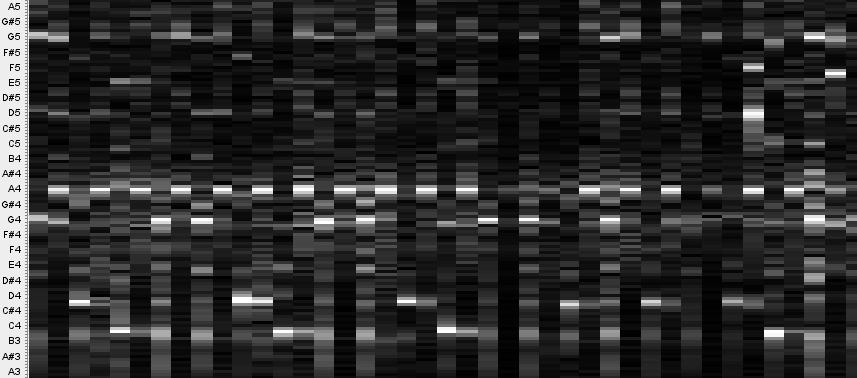
\includegraphics [scale=0.40] {spect_T1c}
  \vspace{20pt}
  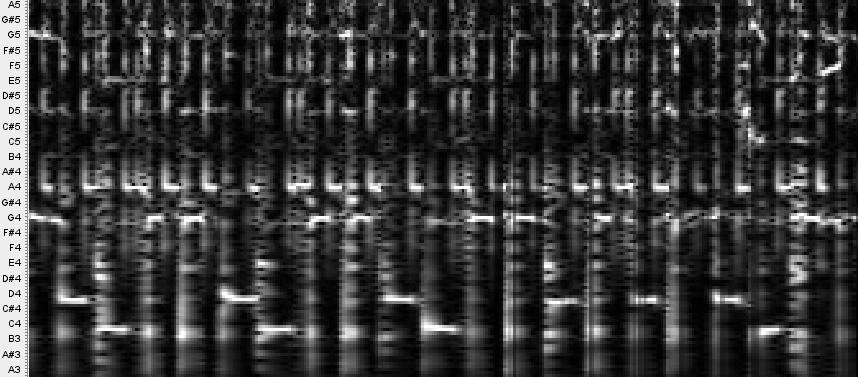
\includegraphics [scale=0.40] {spect_T8c}
  \vspace{10pt}
  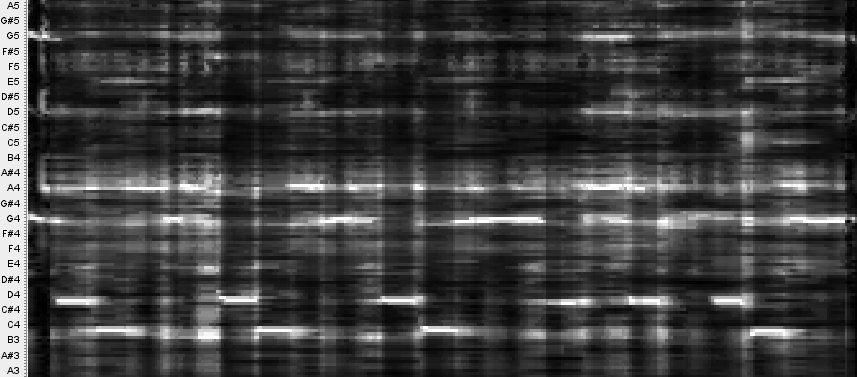
\includegraphics [scale=0.40] {spect_medianc}
  \caption{Фрагменты спектрограммы \emph{The Beatles -- Love Me Do} при $T=1$
  (вверху), $T=8$ (в середине), $T=8$ после сглаживания с $w=19$ (внизу).}
  \label{img:spectT}  
\end{figure}

Равномерно темперированный строй предполагает расположение $N_0=12$ ступеней
звукоряда в пределах октавы, поэтому удобно выбирать $N_0$ кратным $12$. Большие
значения $N_0$ дают возможность в некоторой мере скомпенсировать ошибки при
определении частоты настройки музыкальных инструментов $f_0$, позволяя учесть
близкие к $f_k = 2^{k/12} f_0$ частоты. В \cite{Bello2005}, \cite{Lee2006},
\cite{Mauch2008}, \cite{Oudre2009}, \cite{Cho2010}, \cite{Cho2011}
использовалось значение $N_0=36$. Как показано ниже, $N_0=60$ позволяет добиться
лучшего результата.

\begin{figure}[h]
  \begin{minipage}[h]{0.49\linewidth}
    \center{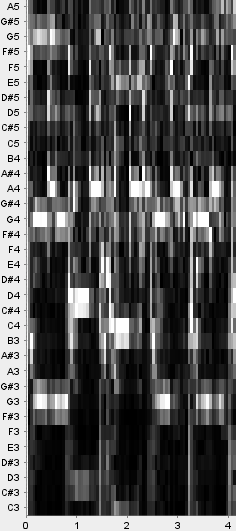
\includegraphics[width=0.5\linewidth]{spect_b12c} \\ а)}
  \end{minipage}
  \hfill
  \begin{minipage}[h]{0.49\linewidth}
    \center{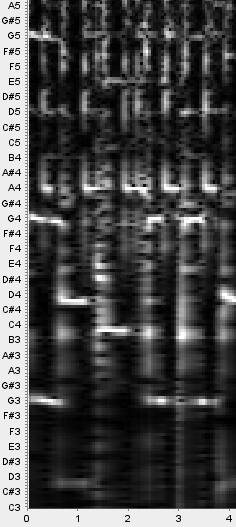
\includegraphics[width=0.5\linewidth]{spect_b60c} \\ б)}
  \end{minipage}
  \caption{Фрагменты спектрограммы \emph{The Beatles -- Love Me Do} при: а)
  $N_0=12$; б) $N_0=60$.}
  \label{img:spectb}  
\end{figure}

Важно также правильно выбрать частоту наименьшей из компонент преобразования
$f_{min}$ и общее количество компонент $N$. Они определяют используемый для
анализа частотный диапазон. Обычно используются частоты в пределах 50-2000 Гц.
В \cite{Weller2009} используемый диапазон ограничен сверху 1000 Гц, а в
\cite{Cho2011} -- 4186 Гц. Для определения более частот ниже 50 Гц требуется
слишком длинный фрагмент звука, а частоты выше 2000 Гц обычно содержат только
гармоники более низких нот, затрудняющие определение аккорда.

В параграфе \ref{ssect3_Tw} анализируется влияние параметров $T$, $w$ и $N_0$ на
качество распознавания аккордов.

% ЭКСПЕРИМЕНТ: сравнение качества распознавания для $N_0$=12,36,60, и охвата в
% 4,5,6 октав.
% ЭКСПЕРИМЕНТ: сравнение с БПФ при тех же условиях (с определением ритма и частоты
% настройки).

%\newpage
%============================================================================================================================

\section{Выделение мелодических компонент спектра и векторы признаков}
\label{sect1_feat}

На этом этапе к спектрограмме применяется серия преобразований. Они нацелены на
акцентирование компонент, которые несут важную для идентификации аккорда
информацию, и на подавление остальных компонент. Наиболее важным является
подавление шума и инструментов с неопределенной высотой звучания, поскольку их
спектр не зависит от звучащего аккорда и сопоставим по уровню со спектром
инструментов, задающих аккорд.

Как видно из рисунка \ref{img:spectT} (в середине), барабан оставляет на
спектрограмме яркие вертикальные полосы. В то же время, гитаре соответствуют
горизонтальные полосы. Это свойство используют алгоритмы разделения звука на
гармонические и перкуссионные компоненты, такие как \cite{Ono2008} и
\cite{Fitzgerald2010}. В данном случае полное разделение является излишним,
необходимо только подавить перкуссионные компоненты.

Маух в \cite{Mauch2010} предложил вычитать из спектрограммы так называемый
фоновый спектр. При этом каждое значение спектрограммы $C_m[n]$ заменять на
$\frac{C_m[n] - \mu_m[n]}{\sigma_m^q[n]}$, где $\mu_m[n]$ представляет собой
среднее значение, а $\sigma_m^q[n]$ -- среднеквадратическое отклонение в
пределах отрезка от $C_m[n-k]$ до $C_m[n+k]$, охватывающего одну октаву, $q \in
\{0, 1\}$. Если полученное значение является отрицательным, вместо него
подставляется 0.

Автором в \cite{Glazyrin2012} было предложено использовать аналог фильтра
Превитт, используемого в обработке изображений для выделения границ. Будем
для каждого фрагмента спектрограммы размера $9 \times 3$ с центром в точке
$C_m[n]]$ вычислять его свёртку с матрицей
$$P = \begin{pmatrix}
-1 & -1 & -1\\
-1 & -1 & -1\\
-1 & -1 & -1\\
2 & 2 & 2\\
2 & 2 & 2\\
2 & 2 & 2\\
-1 & -1 & -1\\
-1 & -1 & -1\\
-1 & -1 & -1\\
\end{pmatrix}$$
Если полученное значение больше 0, то заменим $C_m[n]$ на него, иначе -- на 0.

\begin{figure}[h]
  \begin{minipage}[h]{0.49\linewidth}
    \center{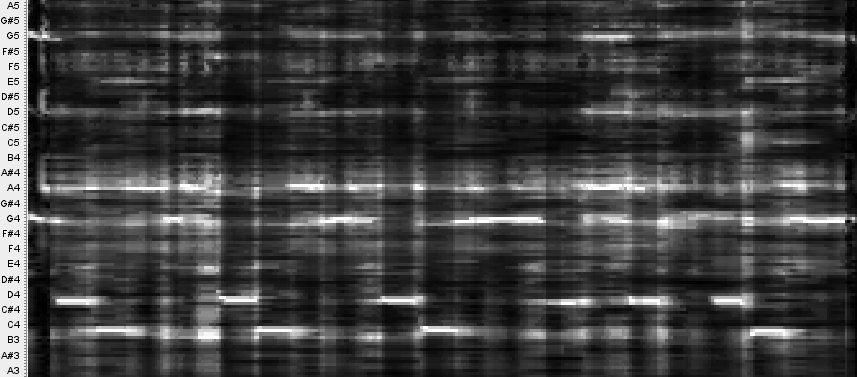
\includegraphics[width=0.9\linewidth]{spect_medianc} \\ а)}
  \end{minipage}
  \hfill
  \begin{minipage}[h]{0.49\linewidth}
    \center{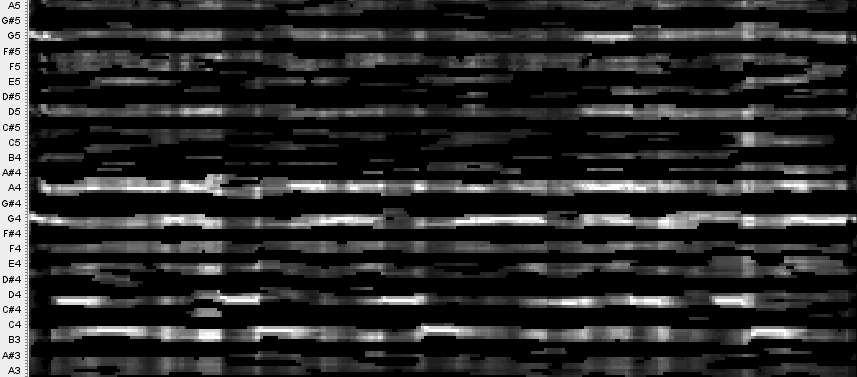
\includegraphics[width=0.9\linewidth]{spect_prewittc} \\ б)}
  \end{minipage}
  \caption{Фрагменты спектрограммы \emph{The Beatles -- Love Me Do}: а)
  до применения фильта Превитт; б) после применения фильта Превитт.}
  \label{img:spectb}  
\end{figure}

Еще один подход к подавлению перкуссионных компонент лёг в основу алгоритма
вычисления признаков CRP \cite{Mueller2009}. Будем рассматривать $C_m[n]$ как
сигнал (количество энергии, приходящейся на данную частоту, в зависимости от
частоты). Применим к этой функции дискретное косинусное преобразование.
$$ DC_m[k] = \sum\limits_{j=0}^{N-1} C_m[j] \cos\left[ \frac{\pi}{N} \left(
j+\frac{1}{2} \right) k \right], \quad k=0, \ldots, N-1 $$
В полученной последовательности значений занулим первые $\xi$ значений, после
чего произведём обратное дискретное косинусное преобразование. Зануляемые первые
коэффициенты соответствуют низкочастотным компонентам сигнала $C_m[n]$, которые,
в свою очередь, соответствуют достаточно длинным последовательностям существенно
отличных от нуля значений. При этом имеющиеся в функции <<острые>> пики
выделяются более чётко.

Как показывает практика, важным шагом является применение к спектрограмме
логарифмического преобразования: каждая компонента $C_m[n]$ заменяется на
$\log_{10}(\eta C_m[n] + 1)$. После него соотношения между компонентами
спектрограммы лучше соответствуют человеческому восприятию интенсивности звука.

В параграфе \ref{ssect3_prewitt} приводится сравнение результатов от применения
различных методов очистки спектра. Параграф \ref{ssect3_crp} посвящён подбору
наилучших параметров для вычисления признаков CRP.

% ЭКСПЕРИМЕНТ: сравнение качества распознавания с применением разных методов
% очистки.

\section{Применение самоподобия} \label{sect1_selfsim}

Важным свойством музыкальных звукозаписей является наличие повторений. Музыка
нравится человеку в том числе из-за повторений одного и того же мотива в разных
вариациях, с некоторыми изменениями. Во многих композициях имеется достаточно
продолжительный повторяющийся припев. В рамках куплета может повторяться одна и
та же музыкальная фраза длительностью в несколько тактов. Можно попытаться
использовать повторения для улучшения спектрограммы.

В работах \cite{Mauch2010} и \cite{Cho2011} повторяющиеся фрагменты композиции
использовались для улучшения качества распознавания аккордов. В обеих методах
строились матрицы самоподобия для 12-мерных хроматических вектороов признаков с
использованием в качестве меры подобия коэффициента корреляции Пирсона (в
\cite{Mauch2010}) и евклидового расстояния (в \cite{Cho2011}). В полученной
матрице находятся линии, параллельные главной диагонали, которые соответствуют
похожим друг на друга фрагментам. Эти фрагменты затем используются для
дополнительного сглаживания спектрограммы.

\begin{figure} [h] 
  \center
  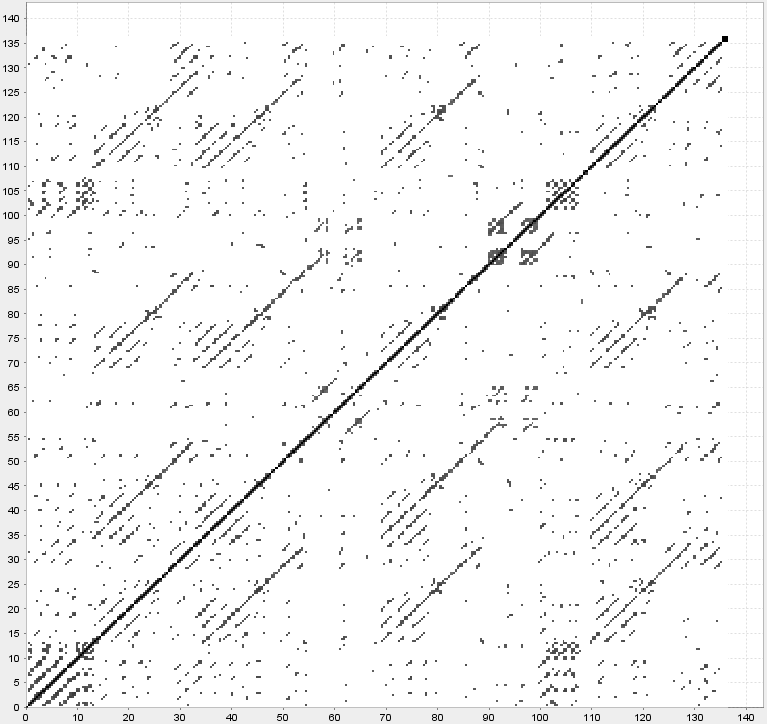
\includegraphics [scale=0.38] {SelfSim}
  \caption{Матрица самоподобия для композиции \emph{The Beatles -- Love Me Do}} 
  \label{img:selfsim}  
\end{figure}

Однако матрицу самоподобия можно строить и для столбцов спектрограммы
$\{C_i\}_{i=0}^{M-1}$, каждый из которых содержит больше информации по сравнению
с соответствующим вектором признаков. Обозначим эту матрицу за $\{s_{ij}\}$, где
$s_{ij}$ -- евклидово расстояние между столбцами $C_i$ и $C_j$. Эта матрица
имеет нули на главной диагонали. Нормализуем её таким образом, чтобы $0 \leq
s_{ij} \leq 1$ для всех $i, j$. Затем в каждой строке сохраняются $\zeta \cdot
M$ наименьших значений ($0 \leq \zeta \leq 1$), а все остальные заменяются на 1.
Пример полученной матрицы показан на рисунке \ref{img:selfsim}.

При помощи полученной матрицы можно скорректировать все столбцы $C_m$:
$$
\widehat{C}_m = \frac{\sum\limits_{j=0}^{M-1} (1 - s_{mj})
C_j}{\sum\limits_{j=0}^{M-1} (1 - s_{mj})} $$

\begin{figure}[h]
  \begin{minipage}[h]{0.49\linewidth}
    \center{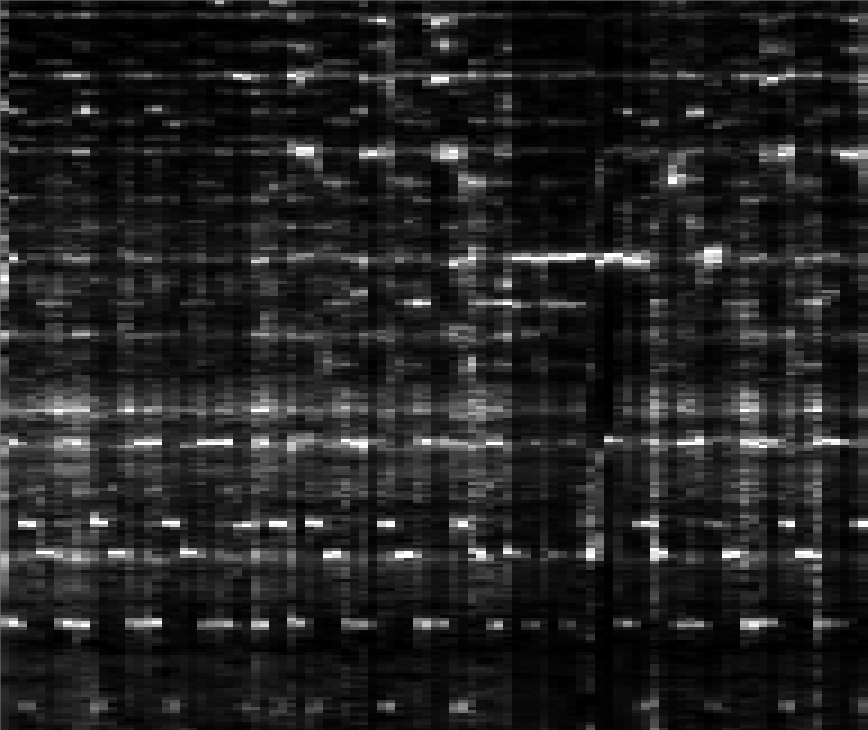
\includegraphics[width=0.9\linewidth]{spect_noSelfSim} \\ а)}
  \end{minipage}
  \hfill
  \begin{minipage}[h]{0.49\linewidth}
    \center{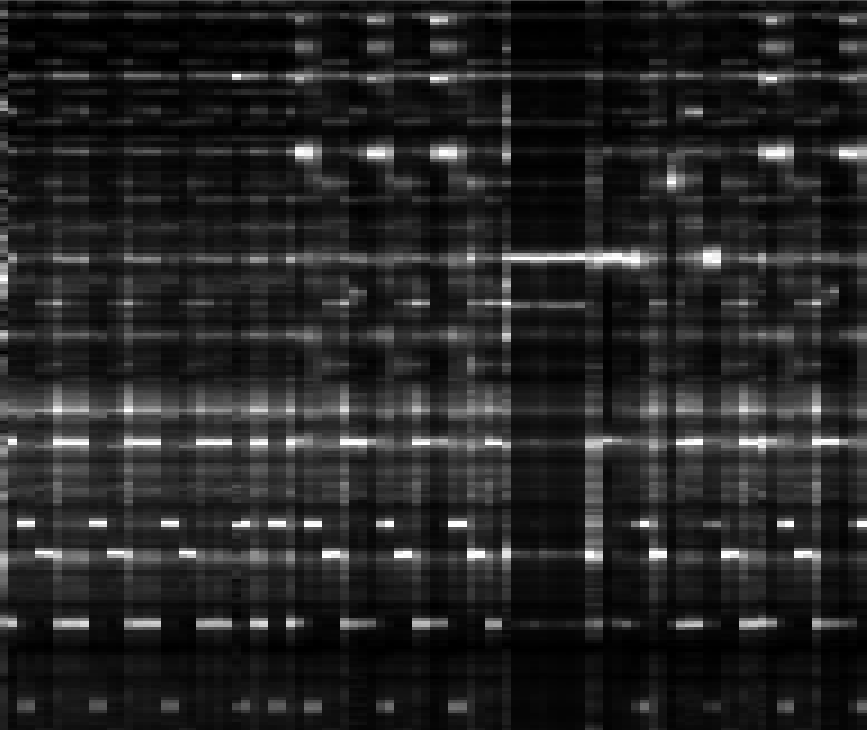
\includegraphics[width=0.9\linewidth]{spect_selfSim} \\ б)}
  \end{minipage}
  \caption{Фрагменты спектрограммы \emph{The Beatles -- Love Me Do}: а)
  без использования самоподобия; б) после коррекции с использованием
  самоподобия.}
  \label{img:spectSelfSim}  
\end{figure}

На рисунке \ref{img:spectSelfSim} наглядно показан эффект от такой коррекции.
Спектрограмма становится существенно чётче, моменты смены аккордов становятся
выделенными более явно. Количественная оценка влияния коррекции на качество
распознавания аккордов приведена в параграфе \ref{ssect3_selfsim}.

Важно, что применение этого преобразования требует наличия достаточно большого
количества столбцов в спектрограмме. Вряд ли имеет смысл применение самоподобия
к короткой звукозаписи, в которой маловероятно наличие повторяющихся элементов. 

% ЭКСПЕРИМЕНТ: сравнение качества распознавания со сглаживанием и без него

%\newpage
%============================================================================================================================

\section{Классификация и исправление ошибок} \label{sect1_class}

\subsection{Классификация хроматических векторов} \label{ssect1_chroma}

Будем рассматривать в качестве множества возможных названий аккордов $Y$ набор
из названий 24 мажорных и минорных аккордов и символа <<N>>, означающего
отсутствие аккорда. За основу возьмём метод ближайшего соседа с шаблонами,
учитывающими основной тон и 3 первых обертона по формуле
(\ref{eq:templates_harmonics}). Эти шаблоны задаются для 12-мерных хроматических
векторов. Столбцы спектрограммы охватывают несколько октав, поэтому для каждого
из них потребовалось бы несколько шаблонов, чтобы учесть все возможные
сочетания октав, в которых могут располагаться ноты аккорда.

% ЭКСПЕРИМЕНТ: зависимость качества распознавания от количества гармоник в
% шаблонах.

Для получения 12-мерных хроматических векторов сначала ко всем значениям
$\widehat{C}_m[n], ~ 0 \leq n < N_0$, прибавляются значения
$\widehat{C}_m[n+N_0], ~ \widehat{C}_m[n+2N_0], ~ \widehat{C}_m[n+3N_0], ~
\ldots$ для каждого $0 \leq m \leq M-1$, давая в результате последовательность
$N_0$-мерных векторов $\{B_m\}_{m=0}^{M-1}$. Далее в случае $N_0=12 b_0, ~ b_0
\geq 3$ каждый вектор $B_m$ преобразуется в 12-мерный вектор $D_m$:
$$ D_m[n] = B_m[b_0 n - 1] + B_m[b_0 n] + B_m[b_0 n + 1], \quad m=0,\dots,M-1,
\quad n=0,\dots,11 $$ 
Для вычисления $D_m[0]$ в качестве $B_m[-1]$ используются $B_m[59]$.

Для каждого из последовательности векторов $\{D_m\}_{m=0}^{M-1}$ определяется
ближайший из шаблонов, и соответствующий ему аккорд считается аккордом, звучащим
в данном фрагменте.

Параграф \ref{ssect3_templates} посвящён подбору наилучших параметров для
используемых шаблонов.

\subsection{Определение отсутствия звучащего аккорда} \label{ssect1_noChord}

Участки, на которых отсутствует звучащий аккорд, не обязательно являются
тишиной. Это может быть также соло на ударных инструментах или какой-либо шум.
Поэтому нельзя определять отсутствие аккорда как близость столбца спектрограммы
или вектора признаков к нулевому вектору. Необходимо каким-то образом учитывать
информацию о наличии и выраженности звуков, соответствующих ступеням звукоряда.

Будем вычислять для каждого столбца спектрограммы следующие величины:
\begin{enumerate}
  \item отношение максимальной по значению из компонент к сумме значений
  всех компонент;
  \item отношение суммы значений компонент, частоты которых в точности
  соответствуют частотам ступеней звукоряда, к сумме значений всех компонент.
\end{enumerate}
После чего будем определять отсутствие звучащего аккорда на фрагменте
звукозаписи, соответствующем данному столбцу спектрограммы, если произведение
указанных двух величин будет меньше некоторого порогового значения $L_{N}$.
Кроме того, будем считать, что аккорды отсутствуют на участках до первой и
после последней из определённых ранее метрических долей.

В параграфе \ref{ssect3_noChord} рассматривается влияние параметра $L_{N}$ на
качество распознавания аккордов.

\subsection{Исправление ошибок классификации} \label{ssect1_errcorr}

В результате экспериментов было обнаружено, что некоторые последовательности
аккордов являются маловероятными в реальной композиции, и скорее всего является
ошибочными. Для двух классов таких последовательностей предлагается метод их
исправления.

\subsubsection{A:maj - A:min}

К первому классу относятся последовательности, в которых аккорды имеют общую
основную ноту, но различные типы, например: A:maj-A:min-A:maj-A:min. Появление
таких последовательностей возможно, поскольку соответствующие векторы признаков
достаточно близки друг к другу. Для каждой такой последовательности находится
вектор признаков, являющийся средним арифметическим составляющих её векторов.
Аккорд, соответствующий полученному вектору признаков, приписывается всей
последовательности.

\subsubsection{A-B-C}

Ко второму классу относятся последовательности из 3 разных идущих подряд
аккордов: A-B-C (при этом возможно A=C). В этом случае более вероятно, что на
самом деле имел место один из следующих 4 вариантов: A-A-C, A-C-C, A-B-B,
B-B-C. Из них выбирается тот, для которого сумма расстояний от векторов
признаков до соответствующих шаблонных векторов минимальна. Очевидно, что такая
коррекция будет ошибочной в тех случаях, когда аккорд действительно звучит
только в течение одной метрической доли.

Эффект от использования предложенных эвристик исследуется в параграфе
\ref{ssect3_heuristics}.

\section{Выводы}

\begin{enumerate}
  \item Разработан метод более точного вычисления спектрограммы, учитывающий
  свойства музыкальных звукозаписей.
  \item Предложен метод для удаления шумовых компонент спектра на основе фильтра
  Превитт, используемого в обработке изображений.
  \item Предложен набор преобразований последовательности векторов признаков,
  учитывающий свойства музыкальных звукозаписей.
  \item Предложены эвристики для исправления распространённых ошибок
  классификации.
\end{enumerate}

%\newpage
%============================================================================================================================

\clearpage			% Глава 1
\chapter{Получение признаков с использованием нейронных сетей}
\label{chapt2}

Описанный в главе \ref{chapt1} метод получения векторов признаков из столбцов
спектрограммы состоит из нескольких преобразований, каждое из которых опирается
на какие-то свойства музыкальных звукозаписей. Представление спектра звука в
виде вектора признаков необходимо, чтобы облегчить последующую классификацию.
Обучение представлениям -- это раздел машинного обучения, рассматривающий
алгоритмы, направленные на получение наилучших представлений входных данных.
Такие алгоритмы стремятся сохранить наиболее характерные признаки входных данных
в сжатом их представлении.

В основе многих алгоритмов обучения представлениям лежит многослойная нейронная
сеть, при обучении которой используются так называемые методы глубокого
обучения. Важным свойством таких методов является возможность предварительного
обучения каждого слоя нейронной сети в отдельности без учителя, на
неразмеченных данных. Во время предварительного обучения параметры каждого из
слоёв достигают значений, более близких к оптимальным, чем при их случайной
инициализации. Благодаря этому для окончательного обучения нейронной сети в
целом требуется существенно меньше размеченных данных, чем потребовалось бы без
использования предварительного обучения. В обзорной статье Й. Бенджио
\cite{Bengio2009} подробно описываются техники, лежащие в основе методов
глубокого обучения.

Методы обучения представлениям впервые были применены к распознаванию аккордов в
звукозаписях в 2012 году: Хамфри в \cite{Humphrey2012} предложил использовать
свёрточные нейронные сети для получения из спектрограммы признаков, позволяющих
классифицировать звучащий аккорд. Этот тип нейронных сетей успешно применяется
при анализе изображений. Фактически, при распознавании аккордов звуковые данные
первоначально также преобразуются в изображение -- спектрограмму. Также
свёрточные нейронные сети применялись для классификации звуков музыкальных
инструментов \cite{Humphrey2011}.

Многослойные рекуррентные нейронные сети были успешно использованы для
распознавания речи в \cite{Maas2012} и для распознавания аккордов в
\cite{BoulangerLewandowski2013}, где нейронная сеть возвращает на выходе
распознанный аккорд, который при помощи рекуррентного соединения подаётся на
вход на следующем шаге.

Хамфри и др. в \cite{Humphrey2013} отмечают, что из-за своей новизны и сложности
методы обучения представлениям и глубокого обучения только начинают
использоваться в различных задачах музыкального информационного поиска. Эти
методы потенциально могут улучшить внутренние представления звуковых данных,
используемые в различных задачах. При этом, в отличие от изображения, звук
меняется с течением времени, что потенциально может быть использовано при
разработке соответствующих алгоритмов.

В данной работе рассматриваются обычные многослойные (в том числе рекуррентные)
нейронные сети, предварительно обучаемые с помощью очищающих автоассоциаторов. В
разделе \ref{sect2_theory} даётся определение многослойного очищающего
автоассоциатора и сопутствующих понятий. В разделе \ref{sect2_sda} описывается
построение и обучение многослойной нейронной сети с использованием
автоассоциаторов, преобразующей столбец спектрограммы в вектор хроматических
признаков.

\section{Теоретические сведения} \label{sect2_theory}

Определения в этом разделе даны в соответствии с \cite{Vincent2010}.

\emph{Автоассоциатор (автоэнкодер)} представляет из себя пару преобразований:
\begin{equation}
y = f_{\theta}(x) = s(Wx+b)
\end{equation}
\begin{equation} \label{g_theta}
z=g_{\theta'}(y) = s(W'y+b')
\end{equation}
Здесь $x$ -- входной вектор, $z$ -- реконструированный выходной вектор, $y$ --
\emph{внутреннее представление} для $x$, $\theta = \{W,b\}$ и
$\theta'=\{W',b'\}$ -- параметры (обычно накладывают ограничение $W'=W^T$), $s$
-- нелинейная функция активации (обычно это сигмоида или функция
гиперболического тангенса). Иногда в (\ref{g_theta}) выбирают в качестве $s$
линейную функцию. Автоассоциатор удобно представлять в виде нейронной сети с
одним скрытым слоем.

При обучении автоассоциатора минимизируется \emph{функция стоимости} $L(X,
Z(X)))$, где $X$ -- множество всех возможных входных векторов. Чтобы в процессе
обучения преобразования $f_{\theta}(x)$ и $g_{\theta}(y)$ не выродились в
тождественные, накладывают различные ограничения. Часто используемое
ограничение: размерность вектора $y$ должна быть меньше размерности входного
вектора $x$. Другой возможный вариант -- потребовать, чтобы размерность вектора
$y$ была больше размерности вектора $x$ и при этом большинство компонент $y$
были равны 0. При этом $y$ становится разреженным представлением вектора $x$.
Обозначим за $f_{\theta}^j(x)$ $j$-ю компоненту вектора $y$ при данном входном
векторе $x$. Тогда можем определить среднюю величину компонент вектора $y$:
\begin{equation}
\hat{\rho}_j = \frac{1}{m} \sum_{i=1}^m f_{\theta}^j(x^{(i)})
\end{equation}
Чтобы добиться $\hat{\rho}_j = \rho$, где $\rho$ -- параметр, контролирующий
разреженность, добавим слагаемое $L_{\rho}$ в функцию стоимости $L$. Это
слагаемое можно определять разными способами, в рамках данной работы будем
использовать следующую его форму, предложенную в \cite{NgCS294A}:
\begin{equation}
L_{\rho} = \beta \left[ \sum_{j=1}^h \left( \rho \log \frac{\rho}{\hat{\rho}_j} +
(1 - \rho) \log \frac{1 - \rho}{1 - \hat{\rho}_j} \right) \right]
\end{equation}
В дальнейшем будем использовать значение $\rho=0.05$, также в соответствии с
\cite{NgCS294A}.

\emph{Очищающий автоассоциатор} обучается таким образом, чтобы по повреждённому
(зашумлённому) вектору $\tilde{x}$ восстанавливать исходный вектор $x$.
Предполагается, что такие представления более устойчивы к помехам и лучше
отражают внутреннюю структуру входных данных. Показано \cite{Vincent2010}, что
во многих случаях внутренние представления, которые получаются при помощи
очищающего автоассоциатора, позволяют получить лучшие результаты в задачах
классификации по сравнению с представлениями, полученными при помощи обычных
автоассоциаторов. В \cite{Vincent2010} рассматриваются различные способы
получения зашумлённого вектора $\tilde{x}$.

\begin{figure} [htbp] 
  \center
  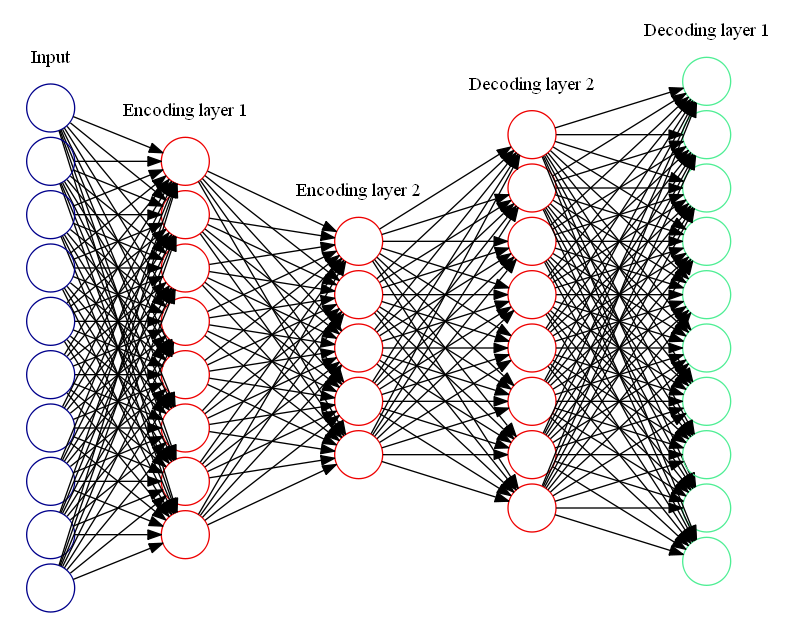
\includegraphics [scale=0.38] {sda}
  \caption{Многослойный автоассоциатор} 
  \label{img:sda}  
\end{figure}

\begin{figure} [htbp] 
  \center
  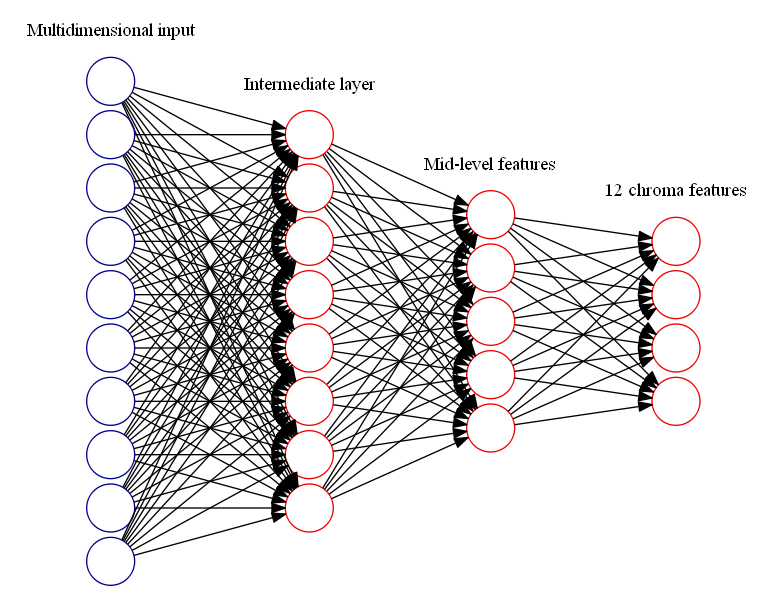
\includegraphics [scale=0.38] {sda_n}
  \caption{Многослойная нейронная сеть} 
  \label{img:sda_n}  
\end{figure}

Из автоассоциаторов можно строить многослойные модели, отождествляя нейроны из
скрытого слоя одного автоассоциатора со входными нейронами другого. Пример такой
модели показан на рисунке \ref{img:sda}. В полученной модели слои можно обучать
друг за другом на неразмеченных данных. Значения, полученные в скрытом слое
последнего из автоассоциаторов, могут быть использованы как векторы признаков.
Пример полученной нейронной сети показан на рисунке \ref{img:sda_n}

Рекуррентный автоассоциатор может быть получен из обычного путём добавления
рекуррентных соединений, связывающих выходы скрытого слоя с дополнительными его
входами, по одному дополнительному входу на каждый выход. Фактически, при этом
получается сеть Эльмана, впервые описанная в \cite{Elman1990}. Пример такой
нейронной сети представлен на рисунке \ref{img:rsda}. Промежуточное
представление $y(x_t)$ в таком случае вычисляется как
\begin{equation}
y(x_t) = s(Wx_t + b + Uy(x_{t-1}))
\end{equation}

\begin{figure} [htbp] 
  \center
  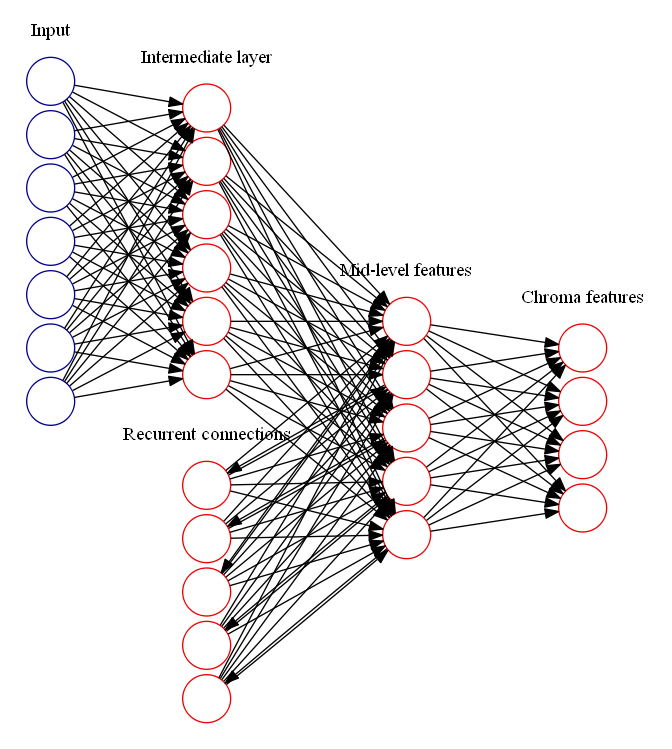
\includegraphics [scale=0.38] {rsda}
  \caption{Многослойная нейронная сеть с рекуррентными соединениями} 
  \label{img:rsda}  
\end{figure}

\section{Построение нейронной сети и предобучение при помощи автоассоциаторов}
\label{sect2_sda}

Существенным недостатком автоассоциаторов является невозможность содержательной
интерпретации значений во внутреннем слое. В частности, невозможно построить
шаблонные наборы значений, соответствующие аккордам. Можно попытаться обучить
алгоритм классификации на векторах значений на выходах внутреннего слоя. Но для
случая 25 классов и достаточно большой размерности векторов для обучения такого
классификатора может потребоваться слишком много данных.

Вместо этого соединим внутренный слой с дополнительным слоем, имеющим 12
выходов. Полученную нейронную сеть обучим на размеченных данных таким образом,
чтобы на выходе получались хроматические векторы (как в разделе
\ref{ssect1_chroma}), в которых каждая компонента соответствует одному
тональному классу. На вход этой сети будут подаваться столбцы спектрограммы.
Таким образом, вместо задачи классификации полученная нейронная сеть решает
задачу регрессии. Классификация же полученных 12-мерных векторов делается как
описано в разделе \ref{ssect1_chroma}.

Предварительное обучение слоёв-автоассоциаторов будем производить методом
мини-пакетного (mini-batch) стохастического градиентного спуска. При этом
сначала обучается первый слой на всём обучающем множестве, затем полученные на
его выходе значения используются для обучения второго слоя, и так далее.
Окончательное обучение сети в целом также производится методом мини-пакетного
стохастического градиентного спуска. При этом в качестве целевых векторов
используются 12-мерные бинарные шаблоны аккордов (описанные в параграфе
\ref{ssectL_nn}), а для случая отсутствия аккорда -- нулевой вектор.
При классификации, соответственно, отсутствие аккорда определяется в случае,
когда ни одна из компонент полученного вектора по абсолютной величине не
превосходит некоторого значения $\Delta$, которое подбирается опытным путём.

Для очищающего автоассоциатора возможные помехи на входе можно моделировать
разными способами. В \cite{Vincent2010} выделяются 3 типа помех:
\begin{enumerate}
  \item аддитивный нормально распределенный шум $\tilde{x}|x \sim
  \mathcal{N}(x, \sigma_0^2 I)$, где $\sigma_0$ -- параметр;
  \item маскирующий шум: некоторые случайно выбранные элементы входного вектора
  обнуляются;
  \item шум типа <<соль-и-перец>>: некоторым случайно выбранным элементам
  входного вектора присваиваются значения 0 или 1.
\end{enumerate}
В случае, когда на вход подаются столбцы спектрограммы, очевидно, более
естественными являются помехи первого типа. В параграфе \ref{ssect3_noise}
исследуется влияние различных типов помех на итоговое качество распознавания
аккордов.

Естественным выбором для функции стоимости будет квадрат евклидова расстояния:
$$L(x,z) = ||x-z||^2$$
Во время предварительного обучения расстояние вычисляется между незашумлённым
входным вектором и выходным вектором. Во время окончательного обучения
расстояние вычисляется между шаблоном аккорда и выходным вектором. Для случая
отсутствия аккорда в качестве соответствующего шаблона используется нулевой
вектор.

В случае, когда в обучающей выборке большинство примеров соответствуют только
одному классу, очень вероятно получить в итоге сеть, которая все векторы будет
классифицировать как принадлежащие этому классу. В данном случае имеется 25
возможных классов, и желательно иметь приблизительно одинаковое количество
примеров на каждый класс. Однако не все аккорды используются в музыке одинаково
часто, и, например, аккорд \emph{до-мажор} может встречаться в обучающей выборке
во много раз чаще, чем \emph{фа-диез-мажор}.

Аналогичная проблема встречается и при обучении скрытых марковских моделей и
байесовских сетей для определения последовательности аккордов по
последовательности векторов признаков. В этих моделях часто используют
циклический сдвиг векторов признаков для усреднения параметров, соответствующих
разным аккордам. Этот процесс подробно описан, например, в \cite{Sheh2003}. Идея
его состоит в том, что, поскольку в хроматическом векторе каждая компонента
соответствует одному тональному классу, его циклический сдвиг даёт вектор,
соответствующий аккорду того же типа (мажорный или минорный) с основной нотой,
сдвинутой на полутон.

В данном случае при окончательном обучении нейронной сети в целом можно также
использовать сдвиг. Но входными векторами являются столбцы спектрограммы, и
циклический сдвиг соответствует неестественному переносу высокочастотных
компонент в область низких частот (или наоборот). Циклический сдвиг можно
заменить простым сдвигом окна соответствующего размера по столбцу спектрограммы,
имеющей охват на одну октаву больше.

При помощи такого сдвига из каждого столбца спектрограммы получается 12
различных столбцов, соответствующих 12 аккордам одного типа с разными основными
нотами. Это позволяет уравновесить количество аккордов в пределах одного типа.
Чтобы уравновесить количество аккордов между типами, потребуем, чтобы в процессе
генерации обучающей выборки из спектрограмм разница между общим количеством
мажорных аккордов и общим количеством минорных аккордов не превосходила
заданного числа $H$.

Во время тестирования также можно использовать циклический сдвиг. Для этого
также для каждого столбца спектрограммы генерируется 12 тестовых векторов, для
каждого из которых при помощи нейронной сети получается хроматический вектор.
Для полученных 12 хроматических векторов производятся соответствующие обратные
сдвиги, а в качестве результата берется среднее арифметическое от полученных
векторов. Эффект от такой модификации процесса тестирования рассматривается в
параграфе \ref{ssect3_cycletest}.

Анализу различных конфигураций нейронной сети и подбору наилучших параметров
посвящён параграф \ref{sect3_nn}.

\section{Выводы}

\begin{enumerate}
  \item Предложен метод для получения хроматических векторов из столбцов
  спектрограммы с использованием предварительно обученной многослойной нейронной
  сети.
  \item Предложен способ для создания обучающей выборки, содержащей
  приблизительно одинаковое количество векторов для всех возможных аккордов.
\end{enumerate}

%\newpage
%============================================================================================================================

% А это две картинки под общим номером и названием:
% \begin{figure}[h]
%   \begin{minipage}[h]{0.49\linewidth}
%     \center{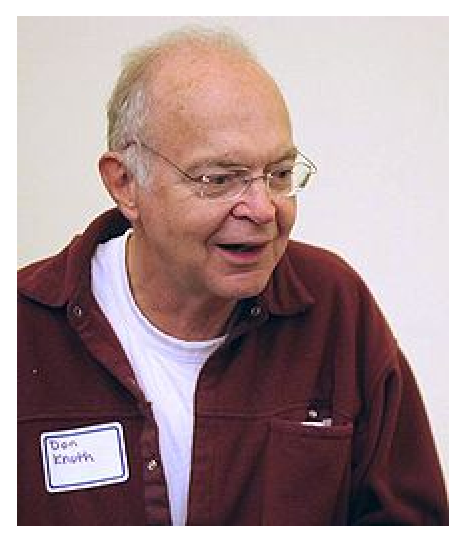
\includegraphics[width=0.5\linewidth]{knuth1} \\ а)}
%   \end{minipage}
%   \hfill
%   \begin{minipage}[h]{0.49\linewidth}
%     \center{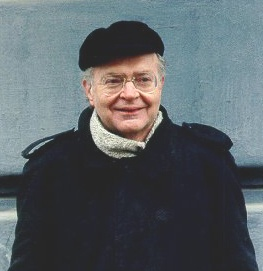
\includegraphics[width=0.5\linewidth]{knuth2} \\ б)}
%   \end{minipage}
%   \caption{Очень длинная подпись к изображению, на котором представлены две фотографии Дональда Кнута}
%   \label{img:knuth}  
% \end{figure}

%\newpage
%============================================================================================================================

\clearpage			% Глава 2
\chapter{Эксперименты} \label{chapt3}

Описанные в главах \ref{chapt1} и \ref{chapt2} алгоритмы имеют значительное
количество параметров. Для подбора их оптимальной комбинации, фактически,
необходимо решить задачу многомерной оптимизации в достаточно большом
пространстве. Очевидно, что в данном случае невозможно решить эту задачу
аналитически. Также невозможно перебрать все возможные комбинации параметров
ввиду слишком большого их числа. Однако во многих случаях можно определить
разумный диапазон возможных значений параметра и исследовать изменение качества
распознавания аккордов в зависимости от значений данного параметра в указанном
диапазоне.

Применение методов вычисления классификации векторов признаков, основывающихся
на машинном обучении, не позволяет целиком избавиться от ручного подбора
параметров. Во-первых, эти алгоритмы могут иметь метапараметры, не изменяемые в
процессе обучения (например, количество нейронов в $j$-м слое нейронной сети).
Во-вторых, параметры имеются также на этапах подготовки входных данных и
интерпретации результата.

Поскольку все эксперименты проводились на описанной в разделе \ref{ssectT_coll}
коллекции из 312 музыкальных звукозаписей, найденные значения параметров будут
оптимальными только для этой коллекции. Способствовать преодолению этой проблемы
могли бы достаточно большие коллекции аннотированных композиций, не существующие
на данный момент.

Все эксперименты можно разделить на 4 группы. В разделе \ref{sect3_spectcalc}
рассматривается этап предварительной обработки звукозаписи и получения
спектрограммы. В разделе \ref{sect3_specttrans} исследуется влияние различных
преобразований спектрограммы на качество распознавания аккордов. Эксперименты
в разделе \ref{sect3_nn} направлены на отыскание наилучших параметров нейронной
сети, используемой для получения признаков. Преобразования над
последовательностями векторов признаков и распознанных аккордов и параметры
выбранного метода классификации анализируются в разделе \ref{sect3_class}. В
разделе \ref{sect3_time} сравниваются скорости работы реализованных алгоритмов.

\section{Оценка качества распознавания аккордов} \label{sect3_eval}

Поскольку алгоритмы распознавания аккордов предназначаются для обработки
музыкальных звукозаписей, необходимо оценивать качество их работы на реальных
звукозаписях, а не на искусственно сгенерированных примерах. Чтобы звукозапись
можно было использовать для оценки, требуется вручную решить задачу
распознавания последовательности аккордов, то есть для каждого момента времени
$t \in [t_{start}, t_{end}]$ указать аккорд $y \in \overline{Y}$, звучащий в
этот момент. При этом набор $\overline{Y}$ включает в себя все возможные в
музыке сочетания нот и отдельные ноты. Также требуется с высокой точностью
указать моменты начала и конца звучания аккордов. Всё это делает задачу
подготовки тестовых коллекций очень трудоёмкой.

Для хранения этой информации используют особым образом отформатированные
текстовые файлы, называемые файлами разметки или файлами текстовых аннотаций.
Ниже приведён пример такого файла:
\begin{lstlisting}
0.000	0.848	N
0.848	1.625	A:min
1.625	3.017	G:maj
3.017	3.895	F:maj
...
\end{lstlisting}
Первый и второй столбцы содержат время начала и конца звучания аккорда
соответственно, в третьем столбце записывается название аккорда. 

\subsection{Коллекции текстовых аннотаций} \label{ssectT_coll}

На текущий момент существует 5 коллекций текстовых аннотаций для популярной
музыки разных исполнителей:
\begin{itemize}
  \item \emph{Isophonics} \cite{MauchOmp2009}. Текстовые аннотации для 180
  композиций (12 альбомов) \textit{The Beatles}, 20 композиций \textit{Queen}
  (с альбома \textit{Greatest Hits}), 18 композиций \textit{Zweieck} (с альбома
  \textit{Zweilicht}). Наиболее часто используется для исследований, несколько
  раз использовалась для ежегодных соревнований MIREX Audio Chord Estimation.
  
  \item \emph{RWC Pop Music} \cite{Goto2002}. Текстовые аннотации для 100
  композиций японской и западной популярной музыки.
  
  \item \emph{Billboard} \cite{Burgoyne2011}. Текстовые аннотации для 197
  композиций из американского чарта \textit{Billboard 100} за промежуток с 1958
  по 1991 год. Использовалась в соревновании MIREX Audio Chord Estimation в 2012
  году.
  
  \item \emph{uspop2002} \cite{Berenzweig2004}. Текстовые аннотации для 195
  композиций американской популярной музыки.
  
  \item \emph{Robbie Williams annotations}. Текстовые аннтоации для 65
  композиций \textit{Robbie Williams} (первые 5 альбомов).
\end{itemize}

Поскольку в аннотациях указывается точное время, важно при анализе использовать
точно те же версии звукозаписей, которые были использованы при подготовке
аннотаций. Это затрудняет использование некоторых коллекций. Для тестирования
алгоритмов в рамках данной работы использовались коллекции \emph{Isophonics} и
\emph{RWC Pop Music}.

\subsection{Сопоставление последовательностей аккордов}

Вопросом оценки того, насколько одна последовательность аккордов (определённая
автоматически) соответствует другой (правильной, определённой человеком),
занимались Харте \cite{Harte2010} и Пауэлс и Питерс \cite{Pauwels2013}.
Последние предлагают следующую конструкцию для определения схожести двух
последовательностей аккордов.

\begin{figure} [h] 
  \center
  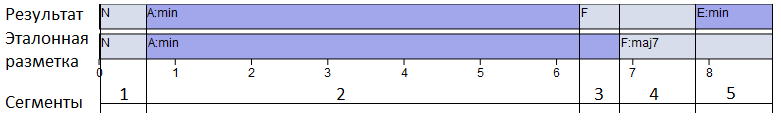
\includegraphics [scale=0.80] {EvaluationSegments}
  \caption{Сопоставление последовательностей аккордов.}
  \label{img:evaluation_segments}  
\end{figure}

Пусть заданы 2 последовательности аккордов: правильная и определённая при помощи
алгоритма. Объединим множества границ аккордов из обоих последовательностей в
одно множество. Используя эти границы, разделим исходную композицию на
сегменты (как на рисунке \ref{img:evaluation_segments}), на каждом из которых
однозначно заданы правильный аккорд $c_{ref}$ и определённый автоматически
$c_{est}$. Пусть также $c_{ref} \in C_{REF}$ -- множество всех аккордов,
встречающихся в аннотациях, а $c_{est} \in C_{EST}$ -- множество всех аккордов,
которые могут быть результатом распознавания при помощи данного алгоритма.

Практически всегда $C_{EST} \subset C_{REF}$, поэтому возникает вопрос о том,
как сопоставлять фрагменты, на которых $c_{ref} \not \in C_{EST}$. Такие
фрагменты можно либо отбрасывать, либо задать сюръективное отображение
$\mathcal{M}: C_{MI} \to C_{MO}$, которое <<сложным>> аккордам из множества
$C_{MI}$ будет сопоставлять <<простые>> аккорды из множества $C_{MO}$. Нужно
выбрать эти множества и отображение $\mathcal{M}$ таким образом, чтобы $C_{EST}
\subset C_{MI}$. Сравниваться при этом будут аккорды $\mathcal{M}(c_{ref})$ и
$\mathcal{M}(c_{est})$. Сегменты, на которых $c_{ref} \not \in C_{MI}$,
отбрасываются. Примером отображения $\mathcal{M}$ может служить отображение,
которое всем аккордам, состоящим из мажорного трезвучия и более высоких ступеней
(например, доминантсептаккорд, нонаккорды и другие) сопоставляет мажорный
аккорд, соответствующий этому трезвучию.

Если необходимо оценить качество распознавания аккордов определенного типа
(например, только трезвучий или только мажорных аккордов), можно ввести
дополнительные множества $C_{LI}$ и $C_{LO}$, ограничивающие соответственно
множества $C_{MI}$ и $C_{MO}$. Тогда аккорды $(c_{ref}, c_{est})$ сравниваются
(не отбрасываются), только если $c_{ref} \in C_{LI} \cap C_{MI}$ и
$\mathcal{M}(c_{ref}) \in \mathcal{M}(C_{LI} \cap C_{MI}) \cap C_{LO}$.

Пусть $\mathcal{S}:C_{SR} \times C_{SE} \to \mathbb{R}^+$ -- функция оценки,
причем $\mathcal{M}(C_{LI} \cap C_{MI}) \cap C_{LO} \subset C_{SR}$ и $C_{MO}
\subset C_{SE}$. Эта функция сопоставляет паре аккордов $\mathcal{M}(c_{ref})$ и
$\mathcal{M}(c_{est})$ неотрицательное действительное число, которое выражает
сходство этих аккордов между собой. Например, можно определить функцию
$\mathcal{S}$ как равную 1 в случае, когда аккорды совпадают, и 0 иначе.

Как видно из \cite{Pauwels2013}, полученные цифры сильно различаются в
зависимости от выбора отображения $\mathcal{M}$ и функции оценки $\mathcal{S}$,
и даже в зависимости от некоторых мелких деталей, таких как способ
синтаксического разбора названий аккордов. Не всегда в статьях корректно
указываются использованные метрики, что делает затруднительным непосредственное
сравнение оценок качества распознавания из статей друг с другом. В этом состоит
главная ценность соревнования MIREX Audio Chord Estimation, где гарантированно
используются одни и те же коллекции и метрики для оценки всех алгоритмов.

В экспериментах в рамках данной работы будем использовать метрику ``Mirex2010''
из \cite{Pauwels2013}. В ней не используется отображение $\mathcal{M}$, а
функция оценки $\mathcal{S}$ строится следующим образом. Сначала $c_{ref}$ и
$c_{est}$ преобразуются в множества тональных классов, для которых находится
пересечение. Обозначим количество элементов в пересечении за $u$.
$\mathcal{S}=1$ в случаях:
\begin{itemize}
  \item $c_{ref}$ является уменьшенным или увеличенным аккордом и $u \geq 2$;
  \item $c_{ref}$ и $c_{est}$ являются символами отсутствия аккорда;
  \item $u \geq 3$.
\end{itemize}
В остальных случаях $\mathcal{S}=0$, то есть $\mathcal{S}:C_{SR} \times C_{SE}
\to \{0, 1\}$. 

Отметим, что при использовании этой метрики ни один сегмент не
отбрасывается. Её выбор является в достаточной степени произвольным и связан
исключительно с тем фактом, что именно она использовалась в соревновании MIREX
Audio Chord Estimation в 2010, 2011 и 2012 годах.

Пусть $\ell_1, \ell_2, \ldots, \ell_{N_{segm}}$ -- длины всех сегментов в
пределах одной композиции, а $s_1, s_2, \ldots, s_{N_{segm}}$ -- соответствующие
значения метрики. Тогда \emph{коэффициент перекрытия (overlap ratio, OR)} для
данной композции определяется как
\begin{equation} \label{eq:or}
OR = \frac{\sum_{i=1}^{N_{segm}} s_i \ell_i}{\sum_{i=1}^{N_{segm}} \ell_i}
\end{equation}
При этом неважно, были ли ceгменты взяты из одной и той же композиции или из
нескольких разных. Но для того, чтобы иметь возможность определить
статистически значимые различия между системами, в экспериментах будем
определять коэффициент перекрытия отдельно для каждой композиции.

Для примера, на рисунке \ref{img:evaluation_segments} $s_1 = s_2 = s_4 = 1$,
$s_3 = s_5 = 0$. На сегментах 1 и 2 аккорды совпадают, на сегменте 4 аккорды
F:maj и F:maj7 имеют 3 общих ступени F, A, C.

Пусть коллекция содержит $N_{tracks}$ композиций, для каждой из которых
вычислен коэффициент перекрытия $OR_k$. Обозначим за $L_i =
\sum_{i=j}^{N_{segm}} \ell_j$ длину $i$-й композиции. Тогда совокупная метрика
для коллекции, называемая \emph{взвешенным средним коэффициентом перекрытия
(weighted average overlap ratio, WAOR)}, вычисляется следующим образом:
\begin{equation} \label{eq:waor}
WAOR = \frac{\sum_{i=1}^{N_{tracks}} OR_i \cdot L_i}{\sum_{i=1}^{N_{tracks}}
L_i}
\end{equation}
Такой же способ усреднения применяется в соревнованиях MIREX Audio Chord
Estimation.

\subsection{Сопоставление границ сегментов}

Метрика для сопоставления границ сегментов была введена Маухом в
\cite{MauchThesis2010}, но не получила широкого распространения. Она позволяет
оценить качество определения границ аккордов алгоритмом, игнорируя при этом сами
названия аккордов.

Пусть заданы 2 разбиения звукозаписи длины $L$ на сегменты $G^0 = (G_i^0)$ и $G
= (G_i)$. Направленное расхождение Хэмминга определяется как:
$$
h(G||G^0) = \sum_{i=1}^{N_G} \left( |G_i^0| - \underset{j}{\operatorname{max}}
|G_i^0 \cap G_j| \right)
$$
где $N_G$ -- количество сегментов в разбиении $G$, а $| \cdot |$ -- длина
сегмента. Оно определяет, насколько $G$ фрагментировано по отношению к $G^0$.
Тогда \emph{сегментация} $H(G, G^0)$ определяется как
$$H(G, G^0) = 1 - \frac{1}{L} max\{ h(G||G^0), h(G^0||G) \} \in [0,1]$$

\subsection{Статистическая значимость}

При сравнении нескольких вариантов алгоритма помимо средних значений метрик
качества необходимо понять, действительно ли между этими вариантами имеются
статистически значимые различия. Для проверки этого предположения будем
использовать непараметрический критерий Фридмана. Он позволяет проверять
гипотезы о различии более двух зависимых выборок. В отличие от дисперсионного
анализа (ANOVA), критерий Фридмана не требует предположений о нормальности
распределения значений метрик для разных композиций, а также одинаковых
дисперсий этих распределений для разных вариантов алгоритма (как отмечается в
\cite{Mauch2010}, эти предположения не является верными в данном случае).

Однако, если в соответствии с критерием Фридмана удаётся отвергнуть нулевую
гипотезу (об отсутствии различий между разными методами), необходимо выяснить,
для каких пар методов имеется статистически значимая разница в качестве
распознавания аккордов. Для этого вычисляется среднее Тьюки (Tukey's honestly
significant difference). В отличие от T-теста, при его допускаются множественные
попарные сравнения. Этот метод используется для сравнения качества работы разных
алгоритмов в рамках всех соревнований MIREX \cite{Downie2008}.

\section{Вычисление спектрограммы} \label{sect3_spectcalc}

На данном этапе необходимо выбрать наилучшие из доступных алгоритмов для
определения ритма и определения частоты настройки. Кроме того, необходимо
определить наилучшие значения для параметров преобразования постоянного
качества: разрешение по частоте $N_0$ (количество компонент, приходящихся на
октаву) и количество октав $N / N_0$, а также для количества вставляемых
промежуточных столбцов спектрограммы $T$ и размера окна при сглаживании $w$.

\subsection{Определение ритма} \label{ssect3_beattrack}

Были рассмотрены 3 алгоритма, позволяющие определить моменты начала метрических
долей в звукозаписи: \emph{BeatRoot} \cite{Dixon2007}, \emph{Beat tracker} от
Дэвиса \cite{Davies2007} (\emph{DBT}) из набора плагинов \emph{Queen Mary Vamp
plugins}\footnote{\url{http://www.isophonics.net/QMVampPlugins}} для системы
извлечения музыкальной информации из музыкальных файлов
\emph{Vamp}\footnote{\url{http://www.vamp-plugins.org/}} и плагина \emph{INESC
Porto Beat Tracking plugin} \cite{Oliveira2012} (\emph{IBT}) для этой же
системы. Выбор алгоритмов обусловлен наличием свободно доступной реализации.
\emph{BeatRoot} дополнительно потребовал небольшого вмешательства в исходный
код для уменьшения потребления вычислительных ресурсов. Кроме того, на 6
композициях из анализруемого набора этот алгоритм не смог определить ритм,
поэтому для этих композиций использовались значения, полученные при помощи DBT.

\begin{table} [htbp]
  \centering
  \parbox{15cm}{\caption{Влияние алгоритма определения ритма на
  качество распознавания аккордов} \label{TBT}}
%  \begin{center}
  \begin{tabular}{|l|l|l|l|}
  \hline
  Алгоритм & WAOR & Сегментация \\
  \hline
  BeatRoot + DBT & 0.7516 & 0.7907 \\
  DBT & 0.7317 & 0.7659 \\
  IBT & 0.7189 & 0.7425 \\
  \hline
  \end{tabular}
%  \end{center}
\end{table}

Наилучшие полученные для данных алгоритмов результаты показаны в таблице
\ref{TBT}. \emph{BeatRoot} показал наилучший результат, статистически значимо
превосходящий результаты, полученные с использованием алгоритмов \emph{IBT} и
\emph{DBT}. Это достаточно удивительно, поскольку первая версия алгоритма
\emph{BeatRoot} была представлена ещё в 2001 году, а в данной работе
использовалась его исправленная версия от 2007 года. При этом \emph{DBT} был
представлен в 2007 году, а \emph{IBT}, схожий по принципу работы с
\emph{BeatRoot}, -- в 2012 году.

\subsection{Определение частоты настройки} \label{ssec3_tunfreq}

Были проведены эксперименты по распознаванию аккордов с использованием
описанного в разделе \ref{ssect1_f0} алгоритма для вычисления частоты настройки
со следующими значениями параметров:
\begin{itemize}
  \item $f_{min} = 220$ Гц, $N_0 = 12 \cdot 20 = 240$ компонент на октаву;
  \item $f_{min} = 220$ Гц, $N_0 = 12 \cdot 10 = 120$ компонент на октаву;
  \item $f_{min} = 440$ Гц, $N_0 = 12 \cdot 20 = 240$ компонент на октаву.
\end{itemize}
Охват во всех случаях составлял 4 октавы. Также для сравнения были проведены
эксперименты без коррекции частоты настройки и с использованием алгоритма,
описанного Маухом в \cite{MauchThesis2010}, раздел 3.1.3 и реализованного в виде
плагина для системы \emph{Vamp}.

\begin{table} [htbp]
  \centering
  \parbox{15cm}{\caption{Влияние алгоритма определения частоты настройки на
  качество распознавания аккордов} \label{TTunFreq}}
  \begin{tabular}{|l|l|l|l|}
  \hline
  Алгоритм & WAOR & Сегментация \\
  \hline
  $f_{min} = 220$ Гц, $N_0 = 120$ & 0.7516 & 0.7892 \\
  $f_{min} = 220$ Гц, $N_0 = 240$ & 0.7516 & 0.7907 \\
  $f_{min} = 440$ Гц, $N_0 = 240$ & 0.7512 & 0.7899 \\
  Маух \cite{MauchThesis2010} & 0.7477 & 0.7888 \\
  -- & 0.7429 & 0.7854 \\
  \hline
  \end{tabular}
\end{table}

Результаты экспериментов приведены в таблице \ref{TTunFreq}. Как видно,
определение частоты настройки приводит к улучшению качества распознавания
аккордов, причем при использовании любого из перечисленных алгоритмов это
улучшение статистически значимо. Использование любого из описанных вариантов
алгоритма из раздела \ref{ssect1_f0} также приводит к статистически значимому
улучшению по сравнению с алгоритмом Мауха, но за счёт большего времени работы. В
то же время между собой эти 3 варианта отличаются незначительно.

\subsection{Разрешение по времени и по частоте, сглаживание}

Вставка между каждыми двумя соседними моментами начала метрических долей
$T-1$ промежуточных значений позволяет повысить разрешение спектрограммы по
времени. Затем, после применения скользящего медианного фильтра с размером окна
$w$ и прореживания в $T$ раз, спектрограмма содержит ровно 1 столбец на каждую
метрическую долю. Ясно, что при больших значениях $T$ имеет смысл выбирать
больше значения $w$ и наоборот. В таблице \ref{TTw} приведены значения для
некоторых комбинаций $T$ и $w$.

\begin{table} [htbp]
  \centering
  \parbox{15cm}{\caption{Влияние параметров $T$ и $w$ на качество распознавания
  аккордов} \label{TTw}}
  \begin{tabular}{|l|l|l|}
  \hline
  Значения параметров & WAOR & Сегментация \\
  \hline
  $T = 2$, $w = 1$ & 0.6780 & 0.7561 \\
  $T = 2$, $w = 3$ & 0.7368 & 0.7830 \\
  $T = 2$, $w = 5$ & 0.7278 & 0.7721 \\
  \hline
  $T = 4$, $w = 5$ & 0.7467 & 0.7886 \\
  $T = 4$, $w = 7$ & 0.7496 & 0.7884 \\
  $T = 4$, $w = 9$ & 0.7451 & 0.7827 \\
  \hline
  $T = 8$, $w = 13$ & 0.7504 & 0.7910 \\
  $T = 8$, $w = 15$ & 0.7516 & 0.7907 \\
  $T = 8$, $w = 17$ & 0.7494 & 0.7863 \\
  \hline
  \end{tabular}
\end{table}

При $T=2$ качество распознавания аккордов существенно хуже для случая $w=1$, что
фактически соответствует отказу от добавления промежуточных значений и
последующих сглаживания и прореживания. Статистически значимых отличий между
вариантами $w=3$ и $w=5$ нет.

При $T=4$ влияние параметра $w$ уже не столь существенно. Наилучший результат
получен при $w=7$, и он статистически значимо превосходит результаты, полученные
при $w=5$ и $w=9$ (разница между которыми, в свою очередь, не является
значимой).

При $T=8$ только разница между вариантами $w=15$ и $w=17$ оказалась
статистически значимой. При этом в абсолютных значениях различия ещё меньше, чем
для $T=4$.

Отдельно было проведено сравнение наилучших вариантов для каждого значения $T$.
Между вариантами $T=4, w=7$ и $T=8, w=15$ нет статистически значимой разницы в
качестве распознавания аккордов; разница в абсолютных значениях метрик также
незначительна. При $T=2, w=3$ был получен существенно худший результат.

Интересно, что наилучшие резултаты достигаются при $w = 2T-1$, что для каждого
момента времени исходной последовательности соответствует фильтрации по
значениям спектра, вычисленным в этот момент и в $T-1$ добавленных промежуточных
точках справа и слева. Из этого эксперимента видно, что увеличение разрешения по
времени для последовательности моментов начала метрических долей по крайней мере
в 4 раза приводит к существенному улучшению качества распознавания аккордов.

\begin{table} [htbp]
  \centering
  \parbox{15cm}{\caption{Влияние параметра $N_0$ на качество распознавания
  аккордов} \label{TN0}}
  \begin{tabular}{|l|l|l|l|}
  \hline
  Значения $N_0$ & WAOR & Сегментация \\
  \hline
  $N_0 = 12$ & 0.6257 & 0.7743 \\
  $N_0 = 36$ & 0.7518 & 0.7951 \\
  $N_0 = 60$ & 0.7516 & 0.7907 \\
  \hline
  \end{tabular}
\end{table}

В таблице \ref{TN0} приведены результаты, полученные при разных значениях
количества компонент преобразования постоянного качества, приходящихся на одну
октаву. Очевидно, что при наличии как минимум 36 компонент на октаву (3
компоненты на ноту) качество распознавания аккордов существенно повышается.
Различия между $N_0=36$ и $N_0=60$ не являются статистически значимыми. Однако
при $N_0=60$ требуется вычислить в 1.8 раз больше значений для компонент
преобразования постоянного качества, а также в дальнейшем многократно вычислять
дискретное косинусное преобразование для большего набора значений.

% Основные вопросы относительно выбора параметров, возникающие на этом этапе:
% \begin{enumerate}
%   \item действительно ли определение частоты настройки музыкальных инструментов
%   повышает качество распознавания аккордов;
%   \item каковы оптимальные параметры алгоритма определения частоты настройки;
%   \item действительно ли определение ритма повышает качество распознавания
%   аккордов;
%   \item есть ли разница между библиотеками \emph{Beatroot} \cite{Dixon2007} и
%   \emph{Beat tracker} \cite{Davies2007} из набора \emph{Queen Mary Vamp
%   plugins};
%   \item возможно ли добиться при помощи быстрого преобразования Фурье и
%   последующего отображения полученного спектра на частоты звукоряда по формуле
%   \ref{fft_wrap} такого же качества распознавания, как при использовании
%   преобразования постоянного качества;
%   \item каковы оптимальные значения для разрешения по частоте $N_0$ (количество
%   компонент, приходящихся на октаву) и количества октав $N / N_0$ в
%   преобразовании постоянного качества;
%   \item каковы оптимальные значения для количества вставляемых промежуточных
%   столбцов спектрограммы $T-1$ и размера окна при сглаживании $w$.
% \end{enumerate}

% \begin{table} [htbp]
%   \centering
%   \parbox{15cm}{\caption{Название таблицы}\label{Ts0Sib}}
% %  \begin{center}
%   \begin{tabular}{| p{3cm} || p{3cm} | p{3cm} | p{4cm}l |}
%   \hline
%   \hline
%   Месяц   & \centering $T_{min}$, К & \centering $T_{max}$, К &\centering  $(T_{max} - T_{min})$, К & \\
%   \hline
%   Декабрь &\centering  253.575   &\centering  257.778    &\centering      4.203  &   \\
%   Январь  &\centering  262.431   &\centering  263.214    &\centering      0.783  &   \\
%   Февраль &\centering  261.184   &\centering  260.381    &\centering     $-$0.803  &   \\
%   \hline
%   \hline
%   \end{tabular}
% %  \end{center}
% \end{table}

\section{Преобразования спектрограммы} \label{sect3_specttrans}

Основные вопросы относительно выбора параметров, возникающие на этом этапе:
\begin{enumerate}
  \item действительно ли применение аналога фильтра Превитт повышает качество
  распознавания акокрдов;
  \item каково оптимальное значение для количества зануляемых первых
  коэффициентов дискретного косинусного преобразования $\xi$ при вычислении
  признаков CRP;
  \item действительно ли сглаживание с использованием матрицы самоподобия для
  столбцов спектрограммы лучше, чем с использованием такой матрицы для векторов
  признаков и без использования самоподобия вообще;
  \item каково оптимальное значение для доли сохраняемых в матрице самоподобия
  значений $\zeta$.
\end{enumerate}

\section{Нейронные сети} \label{sect3_nn}

Для описанного в главе \ref{chapt2} метода получения векторов признаков с
использованием нейронных сетей важными являются следующие вопросы:
\begin{enumerate}
  \item какое количество элементов во входном слое сети позволяет получить
  наилучшие векторы признаков;
  \item влияет ли предварительное применение логарифмического преобразования к
  спектрограмме на полученные векторы признаков;
  \item каковы оптимальное количество скрытых слоёв и их размеры в нейронной
  сети;
  \item действительно ли использование рекуррентных соединений повышает качество
  распознавания аккордов;
  \item каковы оптимальные значения для уровней шума при обучении очищающих
  автоассоциаторов;
  \item и др.
\end{enumerate}

Для проведения экспериментов тестовая коллекция из 318 композиций была случайным
образом поделена на 2 равные части, каждая из которых поочередно выступала в
качестве обучающей и тестовой выборки.

\section{Классификация векторов признаков} \label{sect3_class}

Для выбранного способа классификации векторов признаков необходимо определить
наилучшие значения следующих параметров:
\begin{enumerate}
  \item количество учитываемых при генерации шаблонов гармоник;
  \item степень убывания вклада гармоник в шаблон $s$.
\end{enumerate}
Помимо этого необходимо количественно оценить повышение качества распознавания
при использовании описанных в разделе \ref{ssect1_errcorr} эвристик.

\section{Быстродействие} \label{sect3_time}

\section{Выводы}

\begin{enumerate}
  \item TODO
\end{enumerate}

%\newpage
%============================================================================================================================

\clearpage			% Глава 3: эксперименты
\chapter*{Заключение}						% Заголовок
\addcontentsline{toc}{chapter}{Заключение}	% Добавляем его в оглавление
\label{chaptC}

Основные результаты работы заключаются в следующем.
\begin{enumerate}
  \item На основе анализа \ldots
  \item Численные исследования показали, что \ldots
  \item Математическое моделирование показало \ldots
  \item Для выполнения поставленных задач был создан \ldots
\end{enumerate}
И какая-нибудь заключающая фраза.

\clearpage		% Заключение
\listoffigures									% Список изображений
\addcontentsline{toc}{chapter}{\listfigurename}	% Добавляем на него ссылку в оглавление
\clearpage

\listoftables									% Список таблиц
\addcontentsline{toc}{chapter}{\listtablename}	% Добавляем на него ссылку в оглавление
\clearpage			% Списки таблиц и изображений

% http://tex.stackexchange.com/questions/48005/bibtex-not-showing-using-texlipse
% Добавляем список литературы руками
\addcontentsline{toc}{chapter}{\bibname}	% Добавляем список литературы в оглавление
\bibliography{biblio}						% Подключаем BibTeX-базы

%\input{references}		% Список литературы
\appendix
\chapter{Название первого приложения} \label{AppendixA}

Некоторый текст.

\chapter{Очень длинное название второго приложения, в котором продемонстрирована работа с длинными таблицами} \label{AppendixB}

 \section{Подраздер приложения}\label{AppendixB1}
Вот размещается длинная таблица:
\fontsize{10pt}{10pt}\selectfont
\begin{longtable}[c]{|l|c|l|l|}
% \caption{Описание входных файлов модели}\label{Namelists} 
%\\ 
 \hline
 %\multicolumn{4}{|c|}{\textbf{Файл puma\_namelist}}        \\ \hline
 Параметр & Умолч. & Тип & Описание               \\ \hline
                                              \endfirsthead   \hline
 \multicolumn{4}{|c|}{\small\slshape (продолжение)}        \\ \hline
 Параметр & Умолч. & Тип & Описание               \\ \hline
                                              \endhead        \hline
 \multicolumn{4}{|r|}{\small\slshape продолжение следует}  \\ \hline
                                              \endfoot        \hline
                                              \endlastfoot
 \multicolumn{4}{|l|}{\&INP}        \\ \hline 
 kick & 1 & int & 0: инициализация без шума ($p_s = const$) \\
      &   &     & 1: генерация белого шума                  \\
      &   &     & 2: генерация белого шума симметрично относительно \\
  & & & экватора    \\
 mars & 0 & int & 1: инициализация модели для планеты Марс     \\
 kick & 1 & int & 0: инициализация без шума ($p_s = const$) \\
      &   &     & 1: генерация белого шума                  \\
      &   &     & 2: генерация белого шума симметрично относительно \\
  & & & экватора    \\
 mars & 0 & int & 1: инициализация модели для планеты Марс     \\
kick & 1 & int & 0: инициализация без шума ($p_s = const$) \\
      &   &     & 1: генерация белого шума                  \\
      &   &     & 2: генерация белого шума симметрично относительно \\
  & & & экватора    \\
 mars & 0 & int & 1: инициализация модели для планеты Марс     \\
kick & 1 & int & 0: инициализация без шума ($p_s = const$) \\
      &   &     & 1: генерация белого шума                  \\
      &   &     & 2: генерация белого шума симметрично относительно \\
  & & & экватора    \\
 mars & 0 & int & 1: инициализация модели для планеты Марс     \\
kick & 1 & int & 0: инициализация без шума ($p_s = const$) \\
      &   &     & 1: генерация белого шума                  \\
      &   &     & 2: генерация белого шума симметрично относительно \\
  & & & экватора    \\
 mars & 0 & int & 1: инициализация модели для планеты Марс     \\
kick & 1 & int & 0: инициализация без шума ($p_s = const$) \\
      &   &     & 1: генерация белого шума                  \\
      &   &     & 2: генерация белого шума симметрично относительно \\
  & & & экватора    \\
 mars & 0 & int & 1: инициализация модели для планеты Марс     \\
kick & 1 & int & 0: инициализация без шума ($p_s = const$) \\
      &   &     & 1: генерация белого шума                  \\
      &   &     & 2: генерация белого шума симметрично относительно \\
  & & & экватора    \\
 mars & 0 & int & 1: инициализация модели для планеты Марс     \\
kick & 1 & int & 0: инициализация без шума ($p_s = const$) \\
      &   &     & 1: генерация белого шума                  \\
      &   &     & 2: генерация белого шума симметрично относительно \\
  & & & экватора    \\
 mars & 0 & int & 1: инициализация модели для планеты Марс     \\
kick & 1 & int & 0: инициализация без шума ($p_s = const$) \\
      &   &     & 1: генерация белого шума                  \\
      &   &     & 2: генерация белого шума симметрично относительно \\
  & & & экватора    \\
 mars & 0 & int & 1: инициализация модели для планеты Марс     \\
kick & 1 & int & 0: инициализация без шума ($p_s = const$) \\
      &   &     & 1: генерация белого шума                  \\
      &   &     & 2: генерация белого шума симметрично относительно \\
  & & & экватора    \\
 mars & 0 & int & 1: инициализация модели для планеты Марс     \\
kick & 1 & int & 0: инициализация без шума ($p_s = const$) \\
      &   &     & 1: генерация белого шума                  \\
      &   &     & 2: генерация белого шума симметрично относительно \\
  & & & экватора    \\
 mars & 0 & int & 1: инициализация модели для планеты Марс     \\
kick & 1 & int & 0: инициализация без шума ($p_s = const$) \\
      &   &     & 1: генерация белого шума                  \\
      &   &     & 2: генерация белого шума симметрично относительно \\
  & & & экватора    \\
 mars & 0 & int & 1: инициализация модели для планеты Марс     \\
kick & 1 & int & 0: инициализация без шума ($p_s = const$) \\
      &   &     & 1: генерация белого шума                  \\
      &   &     & 2: генерация белого шума симметрично относительно \\
  & & & экватора    \\
 mars & 0 & int & 1: инициализация модели для планеты Марс     \\
kick & 1 & int & 0: инициализация без шума ($p_s = const$) \\
      &   &     & 1: генерация белого шума                  \\
      &   &     & 2: генерация белого шума симметрично относительно \\
  & & & экватора    \\
 mars & 0 & int & 1: инициализация модели для планеты Марс     \\
kick & 1 & int & 0: инициализация без шума ($p_s = const$) \\
      &   &     & 1: генерация белого шума                  \\
      &   &     & 2: генерация белого шума симметрично относительно \\
  & & & экватора    \\
 mars & 0 & int & 1: инициализация модели для планеты Марс     \\
 \hline
  %& & & $\:$ \\ 
 \multicolumn{4}{|l|}{\&SURFPAR}        \\ \hline
kick & 1 & int & 0: инициализация без шума ($p_s = const$) \\
      &   &     & 1: генерация белого шума                  \\
      &   &     & 2: генерация белого шума симметрично относительно \\
  & & & экватора    \\
 mars & 0 & int & 1: инициализация модели для планеты Марс     \\
kick & 1 & int & 0: инициализация без шума ($p_s = const$) \\
      &   &     & 1: генерация белого шума                  \\
      &   &     & 2: генерация белого шума симметрично относительно \\
  & & & экватора    \\
 mars & 0 & int & 1: инициализация модели для планеты Марс     \\
kick & 1 & int & 0: инициализация без шума ($p_s = const$) \\
      &   &     & 1: генерация белого шума                  \\
      &   &     & 2: генерация белого шума симметрично относительно \\
  & & & экватора    \\
 mars & 0 & int & 1: инициализация модели для планеты Марс     \\
kick & 1 & int & 0: инициализация без шума ($p_s = const$) \\
      &   &     & 1: генерация белого шума                  \\
      &   &     & 2: генерация белого шума симметрично относительно \\
  & & & экватора    \\
 mars & 0 & int & 1: инициализация модели для планеты Марс     \\
kick & 1 & int & 0: инициализация без шума ($p_s = const$) \\
      &   &     & 1: генерация белого шума                  \\
      &   &     & 2: генерация белого шума симметрично относительно \\
  & & & экватора    \\
 mars & 0 & int & 1: инициализация модели для планеты Марс     \\
kick & 1 & int & 0: инициализация без шума ($p_s = const$) \\
      &   &     & 1: генерация белого шума                  \\
      &   &     & 2: генерация белого шума симметрично относительно \\
  & & & экватора    \\
 mars & 0 & int & 1: инициализация модели для планеты Марс     \\
kick & 1 & int & 0: инициализация без шума ($p_s = const$) \\
      &   &     & 1: генерация белого шума                  \\
      &   &     & 2: генерация белого шума симметрично относительно \\
  & & & экватора    \\
 mars & 0 & int & 1: инициализация модели для планеты Марс     \\
kick & 1 & int & 0: инициализация без шума ($p_s = const$) \\
      &   &     & 1: генерация белого шума                  \\
      &   &     & 2: генерация белого шума симметрично относительно \\
  & & & экватора    \\
 mars & 0 & int & 1: инициализация модели для планеты Марс     \\
kick & 1 & int & 0: инициализация без шума ($p_s = const$) \\
      &   &     & 1: генерация белого шума                  \\
      &   &     & 2: генерация белого шума симметрично относительно \\
  & & & экватора    \\
 mars & 0 & int & 1: инициализация модели для планеты Марс     \\ 
 \hline 
\end{longtable}

\fontsize{14pt}{15pt}\selectfont
\section{Еще один подраздер приложения} \label{AppendixB2}

Нужно больше подразделов приложения!

\section{Очередной подраздер приложения} \label{AppendixB3}

Нужно больше подразделов приложения!

\section{И еще один подраздер приложения} \label{AppendixB4}

Нужно больше подразделов приложения!

		% Приложения

\end{document}
